\documentclass{report}
\usepackage{graphicx} % Required for inserting images
\usepackage{amsmath}
\newcommand{\argmin}{\arg\!\min} 
\newcommand{\argmax}{\arg\!\max} 
\usepackage{amssymb}
\usepackage{amsfonts}
\usepackage[T1]{fontenc}
\usepackage{bm}
\usepackage[a4paper, total={6in, 8in}]{geometry}
\usepackage{array}
\newcommand{\lorem}[1]{{\color{red} #1}}
\usepackage{minted}
\usepackage[utf8]{inputenc}
\usepackage{hyperref}
\usepackage{algorithm}
\usepackage{algpseudocode}
\hypersetup{
    colorlinks=true,
    linkcolor=blue,
    filecolor=magenta,
    urlcolor=cyan,
    pdftitle={Overleaf Example},
    pdfpagemode=FullScreen,
    }

\usepackage[
backend=biber,
%style=alphabetic,
sorting=ynt
]{biblatex}
\addbibresource{references.bib}


\title{Simple manipulator control \\
\large A software package for robot control prototyping}
\author{Marko Guberina}
\date{\today}

\begin{document}
\maketitle
\newpage
\tableofcontents
\newpage
\chapter{Introduction}

\section{Purpose}
This text is documentation for a software library for robot control called 
Simple Manipulator Control (SMC). 

The library has 2 purposes:
\begin{enumerate}
\item To speed up the development, testing and deployment
of (primarily) model-based controllers. This is facilitated via the 
``batteries included'' approach, 
by providing a ready-to-use collection of common control strategies.
\item To serve as an educational platform for those looking
	to get into robot control.
\end{enumerate}

These goals are achieved through the following.
The library is developed in Python. This choice allows
for short, flexible, easy-to-understand code, 
a wide array of available external packages,
while still providing real-time control, as heavy computation
is executed in C/C++ via pybind wrappers (via NumPy, Pinocchio etc).
Furthermore, the library is designed to be as simple as possible, 
both in terms of logic,
and the total amount of code. Its skeleton provides a common
interface to both real and simulated robots,
and a wrapper around control loops which are to be written by the users.
The library primarily targets manipulators, but also provides 
support for mobile manipulators,
mainly targeting whole-body control design and testing.

The simplicity comes at the cost of some programming comfort.
This is guided by a personal belief that robotics software 
should get out of the way
of the fact that a robotic manipulator is just 6+ motorized pendulums,
the control of which are easy to implement,
provided appropriate mathematical background.
Thus, the target audience for the library are control engineers
who want to prototype and test their control designs.
More broadly, the target audience  
are people with a more mathematical background
rather than a software background.

Regarding software.
Production-level robotics code should of course not be in Python,
or any language with garbage collection.
However, prototyping control should not have to be done
with the strictest possible software standards,
as this simply takes too much time, and it isn't even clear
that a given controller is worth implementing properly.
Having that said, poorly designed software is the 
biggest hindrance to any project including software.
Thus, the library aims to provide a sensible software architecture,
but without forcing the user to always stick to it.

To further facilitate the educational value
of the library, the documentation explains not only
the control design of existing controllers, but also
the specific software design principles and techniques used.
As mentioned above, software design is essential even for prototyping ---
any code longer than a few hundred lines requires high-level structure
to be useful.

\paragraph{Basic technical information}
\begin{itemize}
\item The library is implemented in Python.
\item The code is tested on MacOS, Arch Linux, Ubuntu 22 and 24, and should work on any Linux. Support for Windows is achieved
 through Docker. The installation procedure for any OS
is documented in the Installation section.
\item All of the robotics-related dependent libraries are written in C++ with Python bindings, proving fast execution despite the Python front-end
		(good enough for real-time control at >500Hz).
\item Most dependencies are optional, and are used only in
	dedicated modules.
\end{itemize}

% TODO: citations on different control strategies listed.
% prolly will mostly be books
\section{Overview of available robot types and controllers}

\paragraph{Available tobot types}
There is basic support for the following types of robots:
\begin{itemize}
		\item single arm manipulators, such as UR5e
		\item dual arm manipulators, such as YuMi
		\item single arm wheeled mobile manipulators
		\item dual arm wheeled mobile manipulators
\end{itemize}
\paragraph{Available controllers}
The library provides the implementation of following common 
velocity-level control strategies for point to
point motions, as well as trajectory tracking:
\begin{itemize}
\item joint space control
\item Cartesian space control via the following inverse kinematics solvers:
\begin{itemize}
	\item Jacobian-based solvers such as damped Jacobian pseudoinverse
	\item various QP formulations
\end{itemize} 
\item impedance control
\item optimal control in the form of trajectory optimization (including MPC)
\item dynamic motion primitives (DMP)
\end{itemize}
There is also some existing functionality for motion planning
\begin{itemize}
	\item path planning
\begin{itemize}
	\item dynamical system-based planning
	\item random path generation
\end{itemize} 
	\item interpolation
\begin{itemize}
	\item approximating B-splines
\end{itemize} 
	\item trajectory generation (ongoing work)
\begin{itemize}
	\item polynomial trajectories
\end{itemize} 
	\item visual servoing (ongoing work)
\end{itemize}

Future work consists of the following:
\begin{itemize}
	\item joint and Cartesian space torque-level control
\item controllers for extrinsic dexterity
\end{itemize}


\subsection{Supported robots}
\begin{itemize}
  \item UR robots
  \item ABB YuMi
  \item ABB mobile YuMi
  \item Sleipner + YuMi platform (SLuMi) 
  \item MiR mobile base with a UR arm (Heron)
\end{itemize}
Every robot, and its interface, has particular quirks
one has to be aware of when working with hardware.
To the extent pertinent for the library,
they are described in \ref{chapter-hardware}.

Planned extension of support:
\begin{itemize}
\item Franka Emika
\item KUKA LBR iiwa
\end{itemize}


\paragraph{Extending support to other robots}
Detailed instructions for extending to other robots are 
provided in Appendix \ref{sec-supportable-hardware}
but it consists of the following steps:
\begin{itemize}
\item Robot models are loaded via URDF.
\item The communication interface with the robot is achieved through either:
\begin{enumerate}
\item A direct interface, ex. socket with a protocol.
The interface has to contain functions for reading of the robot's state (joint positions, velocities, f/t sensor as vectors)
  and functions to send control inputs (joint velocities).
\item ROS1 driver. Due to ROS1 depending on deprecated 
	Python versions, the ROS1 driver is to run in a Docker
	translation layer, while communicating
	with SMC though protobuf-serialized messages over sockets.
\item ROS2 driver. The appropriate robot's ROS2 Node inherits
	SMC's RealRobotManager, providing both SMC and ROS2 functionality.
	In addition, in main files the controllers need to be registered
	instead of immediately executed,
	but otherwise everything is the same.
\end{enumerate}
\item Interfacing with grippers is dealt with on a case-by-case basis
	depending on the specific hardware setup and available drivers.
	Strong preference is given to independent gripper drivers
	as this allows for simultaneous control of the robot and
	the gripper.
\end{itemize}

\section{Usage instructions}
The best way to get a hang of the library is by looking at
the examples available in the \fbox{\texttt{examples}}
directory.
Different arguments and script description is available through 
\newline
\fbox{\texttt{python examples/script.py --help}}.
More involved examples come with a technical report explaining the 
goal of the example and how it is achieved.

The library itself is documented within this document.
This concerns the high-level design decisions,
and the most important elements.  
The \textbf{code itself is documented} and users are highly encouraged 
to look into it, as it can often be used as a starting point
when developing new functionality.

The available control designs are briefly introduced in the control chapter.
In those, the reader is referred to books and 
papers for their theoretical background.
Every controller comes with its example script,
and with an instruction of how to run it in
the \textbf{How to run} paragraphs, which denote where
the example is and which arguments are important for it.
The same is true for various robot classes.

A \textbf{suggested workflow} for writing new examples
and expanding the library can be found in the 
\ref{sec-suggested-workflow} section.

For users with little experience with Python, Linux and similar
topics there are references to relevant learning material 
in the Dependencies section. The idea is to provide 
the minimum working knowledge needed to write
a new controller and test it on hardware.

\chapter{Installation}
\section{Software dependencies}
Tutorials and documentation of the dependencies is
provided in the following chapter. Here they are simply
listed for the purposes of installation.
\begin{itemize}
\item any Linux OS, MacOS or Docker on Windows+WSL
\end{itemize}
Python packages:
\begin{itemize}
\item Pinocchio - robot math
\item NumPy - math
\item matplotlib - plotter, log analysis
\item meshcat, meshcat\_shapes - visualizer (NOTE: will be replaced with viser in the future)
\item (optional) ur\_rtde - UR robots interface 
\item (optional) ROS2 - YuMi, Mobile YuMi, and Heron interface
\item (optional) Docker - SLuMi (to build the translation layer image)
\item (optional)  qpsolvers, quadprog (default solver), proxsuite, ecos, pin-pink (uses quadprog under the hood) - ik solvers
\item (optional) crocoddyl - opc/mpc: 
\item (optional) casadi (requires pinocchio > 3.0) - altertive ocp 
\item (optional) shapely - dynamic system based path planning
\item (optional) opencv-python - visual servoing 
\item (optional) pyqt6 - path input via drawing
\item (optional) protobuf - networking
\end{itemize}

\section{Installation steps}
\subsection{Python package - pip}
You can install all 
dependencies with conda or pip and then do a local pip install of SMC.
conda is the most reliable method as Pinocchio and Crocoddyl
ship primarily through conda-forge
\fbox{\texttt{conda install pin -c conda-forge}}.
Other packages can then 
be installed either with conda or pip.

Look in the Dockerfile for specific package names, 
or consult the list above. Conda and pip installations 
are ocassionally manually tested
on Ubuntu 22 and 24, Arch Linux and MacOS. 
Empirically, Ubuntu WSL on Windows works as well as a 
normal Ubuntu installation.

The library itself is in the python/smc directory. 
Navigate to python directory and do a local pip install with 
\fbox{\texttt{pip install -e .}}

\paragraph{Author's note 1} 
A file specifying the exact dependency versions is explicitely not provided.
This is because it has to be continuously updated to be correct, 
and SMC's author does not have the time for this. 
Additionally, unless you are creating 
a new virtual environment for every project,
you will likely have to manually manage 
versions of Python packages sooner or later.
Moreover, you are expected to be(come) 
familiar with the dependencies due to how heavily
they are relied upon in the codebase, and their use in writing new code.
You are forced to at least manually copy-paste 
to install them as a pedagogical measure
(on top of the lack of the author's time to properly maintain the code). 

\paragraph{Author's note 2}
If you are not running Linux (be it native, or in Docker or on WSL), 
there is a high likelihood of
something not installing or working correctly. 
This is because some dependencies 
are compiled (only) on Linux and are not available on other platforms 
or do not have even have ports to other OS's.
In general support for Linux is much better as it is 
the de facto OS of choice in robotics,
and is also much poorer than in other areas due 
to a compartively low number of users.
Manual compilation of those dependencies is guaranteed to be much more work
than learning the basics of Linux's CLI and using Docker.

\subsection{Virtual machine - Docker}
In the interest of time and convenience, the library is shipped as a Docker image.
This is primarily so that the user does not have to install
Linux on hardware to use the library (although that is the
best option if possible).
Here the operational steps are listed, but there
is a short introduction to Docker in the Dependencies chapter.

\subsubsection{Installing Docker on Windows}
\begin{enumerate}
\item install wsl with "wsl --install" in powershell administrator, more at \href{https://learn.microsoft.com/en-us/windows/wsl/install}{windows docs}
\item install docker on windows (with wsl option, should be default), more at \href{https://docs.docker.com/desktop/install/windows-install}{Docker docs}
\item create the docker account 
\item open docker desktop, navigate to Settings (by user/account button) -> Resources -> Network -> click on enable host networking
\end{enumerate}

\subsubsection{Installing Docker on MacOS}
\begin{enumerate}
\item go to [docker webpage](https://docs.docker.com/desktop/setup/install/mac-install/). 
   select the docker for your processor (intel or apple silicone).
   download and install docker-desktop.
\item if using user-level installation, add docker commands to path with 
		\newline
		\fbox{\texttt{export PATH=[path\_to\_docker\_bin,ex /Users/yourusername/.docker/bin]:\$PATH}}.
   put this into your .bashrc or .zshrc if you don't want to do it every time you start the terminal (it's just another environment variable).
\item create the docker account 
\item open docker desktop, navigate to Settings (by user/account button) -> Resources -> Network -> click on enable host networking
\item extra step to open windows from docker: 
		\begin{enumerate}
				\item install xquartz from \href{xquartz.org}{xquartz.org}. 
						this is needed for real-time-plotting and 
						other graphs to be shown
   (they need to open a window to do that). 
\item reboot after installing for the program to take effect.
\item   then you start the xquartz app. it won't open any window, but in the top-left corner you will see its name (next to apple logo).
   clik on that, go to settings -> security -> clik on "allow connections from network clients" (the docker container will use the localhost network 
   to interface). 
\item you need to reboot again for this to take effect.
		\end{enumerate}
\end{enumerate}


\subsubsection{Building or pulling the SMC Docker image}
Here are the steps to get to your container running once Docker is installed.
You can either build the image locally or pull it from our server (better because it won't take long).
To proceed you need to have the Docker desktop GUI app running (open).

\paragraph{ Building the image locally}
\begin{itemize}
\item [WINDOWS] open wsl (type wsl in powershell) and navigate to git folder (now in wsl) with 
		\newline
		"cd /mnt/Users/YOURUSERNAME/PATH\_TO\_GIT\_FOLDER"
\item [MAC] open a terminal and navigate to git folder with 
		\newline
		"cd /mnt/Users/YOURUSERNAME/PATH\_TO\_GIT\_FOLDER"
\item build the image with "docker build -t smc -f docker/Dockerfile ." NOTE: if you are on mac and have an apple silicone processor,
    you might need to change the ubuntu version to one that works on the apple silicone processor.
\end{itemize}

\paragraph{Pulling the image}
\textbf{TODO: docker pull is depricated, server needs to be updated}.
\begin{itemize}
\item login to our docker server with "docker login docker.control.lth.se -u docker\_repo" with password "repo\_Docker"
\item pull the image with "docker pull 
\end{itemize}

\paragraph{Using the image}
\begin{enumerate}
\item   [Linux and MAC]: NOTE: FIRST RUN \fbox{\texttt{xhost +}} EVERY TIME before you run the image. otherwise docker can't open new windows,
   so real-time-plotting won't work. 
\item [MAC] you need to have xquartz installed to have the xhost + command (look at installation for more).
   NOTE! if you don't get real-time-plotting with xhost +, do xhost + 127.0.0.1 and replace -e DISPLAY=\$DISPLAY with 
   -e DISPLAY=127.0.0.1:0 .
\item to run the image run 
		\newline
		\fbox{\texttt{docker run --rm -it --net=host -e DISPLAY=\$DISPLAY -v /tmp:/tmp smc /bin/zsh}}
\item   [WINDOWS]: NOTE: i've been told that mapping the /tmp folder is not necessary on windows and that it in fact might cause problems.
   in this case just remove the "-v /tmp:/tmp" from the command
\item verify installation by running an example with --visualize-manipulator and --real-time-plotting arguments
\item if you want to make persistent changes to the code from the docker, you need to use the -v argument in docker run to share the folder
   with the code between your native OS (host) and the docker container. 
   in particular, use 
   \newline
   \fbox{\texttt{-v [path\_to\_folder\_on\_host]:[path\_to\_that\_folder\_in\_docker\_container]:rw .}}
   notice the :rw at the end. this allows for both the host and the container to modify the files (otherwise they will be read-only).
\end{enumerate}

\paragraph{MacOS note}
Unfortunately, --net=host does not work on Mac. You will have to bind the 7000 port where Meshcat (visualizer for SMC) appears
with -p 127.0.0.0:7000:7000 . If Meshcat opens new ports (7001, ...) because it didn't close properly, killall python3 should get rid
of the non-closed ports. Alternatively bind a series of ports, say 7000-7010 for slightly more convenience.

\paragraph{Specific usage advice}
Do not change library code, or write your example in the examples directory.
These are owned by the image, and no changes to them will be saved.
If you want persistent changes there, you will need to rebuild the image.
This is almost certainly avoidable and completely unnecessary. 
Instead, map a directory on your host OS (or wsl) to a directory on the image,
and give it read-write privileges. This way you can work on your code
normally, and you don't have to rebuild the image.
The change you think is necessary to some RobotManager or ControlLoopManager can almost 
certainly be achieved with an external function, and be applied
in a custom controlLoop.
Of course, if you think it is valuable to more than yourself,
contact me, I would love to integrate your functionality into the library itself.

\paragraph{Installing additional software on the image}
Install things as you would normally (using apt in the terminal etc).
To get this to be a part of the Docker image, just use
the RUN [...] command in the Dockerfile, where you replace [...] with the
command you used to install what you installed normally.
Don't forget to build the image to apply these changes!
I highly recommend adding software this way, because
it will allow you to share the exact same set-up between your colleagues,
which will help you avoid headaches in the future.

NOTE that if you build many images docker will very quickly use up a lot of your hard drive. 
It does this because it saves the 
To solve this

\subsection{Native installation (installing ubuntu)}
\begin{enumerate}
\item Either create a disk partition for Ubuntu on your hard drive, or use an external hard drive. In the first case, you might need to shrink your existing partition. Searching for "how to create a disk partition [your\_OS]" or "install ubuntu on [your\_OS]" will get you all the information you need. Ideally, back up your data before any of this (you should be doing this in general as it's good practice).
\item Download an Ubuntu 22 LTH iso (file which contains everything needed for installation), available at official Ubuntu websites
\item Create a bootable USB. In short, you can't just copy an iso file to a USB and boot from it. Just google how to do it on your OS (use rufus if on windows).
\item Enter BIOS to ensure you can boot from your USB. Ideally this step should just be to enable Boot menu, but this step is dependent to a specific computer. Any reasonable Ubuntu (or any Linux) installation guide should have detailed steps, but also consult your laptop manufacturer websites for BIOS steps if the steps won't be obvious/easy to follow.
\item Boot from the Ubuntu USB and install it to the partition/external disk from step 1. MAKE SURE you are installing to the right partition. To select the partition, select the "Advanced installation" option (selecting the partition is the only advanced thing you need). Otherwise just follow the installation instructions you get once you boot into the USB, they are quite well done.
\end{enumerate}

\section{Installing along with ROS2}
Since ROS is very easy to completely break during normal usage, you are strongly encouraged to use virtualisation.
This is especially valuable when switching ROS versions.
The most common and reliable virtualisation option in this case too is Docker.
Having that said, ROS Docker containers still rely on an Ubuntu host to actually work
(you have been warned if you try using a different host distribution).
Thankfully, in the case of Windows, Ubuntu on WSL will be OK.

Regarding the SMC-ROS Docker installation which also covers installation
of drivers for supported robots, look into the supported hardware appendix.
If you are extending SMC to a new robot running ROS,
read the following subsection.


\subsection{ROS containers repo}
An amazing resource to set up a Docker image with ROS is
\href{https://git.cs.lth.se/robotlab/ros-containers}{ROS containers}
developed at Lund University's Computer Science department.
It does a batteries-included installation of ROS in Docker
and of Docker itself.
It shares the home directory with the host system by default,
and makes the image persistent.
There it is easy to do a native Linux installation of SMC.
Just \textbf{note} that you should do a non-virtualised
installation of Python dependencies as working virtualised
Python environments and ROS is very annoying,
and yields you no benefits (just make one more container 
in case of conflicting packages).

Otherwise, if you prefer managing Docker yourself,
you may write a Dockerfile which uses
an image with Ubuntu with ROS as a starting off point
and adding in the SMC part.
You can probably get away with simply copy-pasting
from the ROS-less Docker image for SMC.

\chapter{Required prior knowledge}

\section{Assumed prior knowledge}
The target audience are engineering students.
We assume Bachelor level engineering knowledge of mathematics,
physics, programming and control.
The list of required topics is given below,
followed by some key concepts from said topic.
%A simple litmus test for whether you know enough is the following.
%Say I give you a URL to a csv file which contains
%the points of a n-dimensional quadratic function.
%Can you need to find the minimum of this function?
%This would entail that you open an empty Python file, 
%download the file and load the points, 
%do a least-squares fit of a quadratic on them,
%and then either implement vanilla gradient descent 
%or explicitly compute the minimum by solving for x at gradient 
%equal to zero (and knowing why both of these work.)

\begin{itemize}
		\item (multivariate) calculus: partial derivatives, gradients,...
		\item linear algebra: matrix inverse, nullspace...
		\item mechanics: dynamics, Lagrangian mechanics
		\item basic convex optimization: convex functions, 
				gradient descent,...
		\item basic programming: OOP concepts, algorithm complexity,...
		\item introductory control course: error dynamics,  
				stability, PID control,...
\end{itemize}


\section{Topics covered in pre-requisites tutorials}
In order to work with robots, you will need to some
very basic operating systems (OS) concepts.
The target OS is Linux as it the standard in robotics,
but the topics covered apply to any OS.
In order to work with the library, you will need to know
how to program in Python and some experience
with a few important packages such as NumPy.
Since these are not always covered outside of a
computer or data science curriculum,
dedicated tutorials have been developed to fill in the gaps.
All of these topics are covered in the context of
the SMC library and robotic control with concrete examples.

Following the pre-requisites there are dedicated
tutorials on using SMC. Finally, 
there is a small crash introduction to Lie algebra for robotics,
and a crash introduction to project management as
even small robotics projects can get very convoluted,
very fast, if one is not careful and deliberate.

Tutorials on Linux, Python and the SMC library 
are in 
\href{https://gitlab.control.lth.se/marko-g/LPR-tutorials}{LPR tutorials}.
These tutorials are in both text and video formats 
(TODO atm the text is only a list of topics, while
the videos are actual tutorials).
Just the videos can be found in the following 
\href{https://www.youtube.com/playlist?list=PLKOlTxWSIaGWsaJwz6oKtgGB1Ukv_RIeP}{YouTube playlist}.

The tutorials aim to give you an overview of the topics,
tell you only the essential information, and refer you
to other resources for anything else. You might need
all of them, or none of them --- have a look to be sure
you're covered.
The topics covered, and the main goal are:
\begin{itemize}
		\item The GNU/Linux command line interface (CLI) - 
				navigating directories, installing packages
		\item Docker - (special) virtual machines,
				building images (SMC Docker image) and running
				containers
		\item Networking - IP address and ports, creating
				new connections (creating a manual fixed-IP connection
				to the robot), basic debugging
		\item Python - syntax, standard library and some gotchas,
				basic packages like NumPy, matplotlib, SciPy
		\item Multiprocessing - most basic inter-process communication
				(IPC), running a function in parallel in Python
		\item Computer vision - common modern approaches
				and short introduction to OpenCV
		\item Robotics - high level description
				of what a robot is and basic control 
				approaches
		\item Lie algebra - concepts required to understand
				robot kinematics - \textbf{it's easier
				to learn this than to try to avoid it}
		\item SMC - intro and overview, Pinocchio
				(package for robot math),
				tutorial on leveraging exiting controllers,
				tutorial on writing a new controller
		\item Project management - project planning,
				iterative prototyping, software management with git
\end{itemize}
There is also bonus content for some of the topics
to try to convince you that it's worth it to dig
a bit deeper.

Books, websites and documentation of other topics will be provided 
as they appear in the text.


\section{Robotics}
\label{sec-robotics-into}
This section is by absolutely no means a proper
introduction to robotics. 
For this the reader is referred to the following books:
\cite{murray,lynch}.
In particular the following chapters:
\begin{itemize}
		\item TODO: Lynch, list key chapters
		\item TODO: Murray, list key chapters
		\item \href{https://scaron.info/robotics/jacobian-of-a-kinematic-task-and-derivatives-on-manifolds.html}{this excellent blog post}.
\end{itemize}

%The twist $ V_{ \text{error} }  $ 
%corresponds to the velocity such that moving 
%from frame $ \left\{ e \right\}    $, with twist $ V_{  e}  $, for
%one unit of time, leads to the $ \left\{ g \right\}   $ 
%frame.
%Said another way, if $ \left\{ V_{  e} \right\}   $ is
%the body velocity of the end-effector frame for one unit
%of time, it gets to the goal frame.
%The reason this works has to do with Lie algebra.
%Detailed overview can be found in ex. 
%Frank C. Park, Kevin Lynch - Modern Robotics
%or Murray, R.M., Li, Z. and Sastry, S.S., 2017. A mathematical introduction to robotic manipulation. CRC press,
%or on 
%\href{https://scaron.info/robotics/jacobian-of-a-kinematic-task-and-derivatives-on-manifolds.html}{this excellent blog post}.

However, we can not allow perfection to be the enemy of good.
Going through a robotics course and reading a few introductory 
books is objectively speaking not a hard requirement 
to get into robotics and robot control.
This is because we can leverage software to hide and 
automatically deal with many of the robotics concepts
and math. Just as one does not need to have read the
TCP standard and the rest of RFCs in order to open
a web browser and search the internet.
Having that said, working with robots is much more
involved than searching for recipes online,
and some amount of technical detail is simply unavoidable.
This is especially the case for engineers working with robots.
Also, knowledge is power, and the more knowledge you have,
the more you can do.

The purpose of this section is to at least lay out
the basic concepts and terminology required to specify 
a task for the robot. Additional mathematical detail
is laid out in the Control section \ref{sec-control}.
Depending on what you're trying to achieve you'll need
none of that, or it won't be nearly enough.
Hence it is advised to follow a top-down approach, 
i.e. to utilize the concepts described here and the 
ready-made controllers until this stops being enough the problem at
hand, at which point one should dig into the underlying math
to get a good understanding of what's happening.

\subsection{Basic terminology}
\label{sec-robotics-terminology}
A robot is series of \textbf{actuators} (motors) connected with 
\textbf{links}. For the purposes of this text, all
links are \textbf{rigid} and the motors work perfectly
(no friction, instantaneous reference reaching).
A robot \textbf{joint} is a combination of an actuator
and a link --- basically the robot's equivalent of limb.
In the case of a rotational motor we have
a revolute joint whose position is described in radians.
A series of joints creates a \textbf{kinematic chain}.
If only one end is ``bolted'' to a table or floor,
while the other is free, we call it an \textbf{open kinematic chain}.
Otherwise, it is a \textbf{closed kinematic chain}.
An open kinematic chain robot consisting of revolute joints
is referred to as a \textbf{robotic manipulator} (more or less).
Thus one might consider a quadruped a combination of 4 manipulators,
which form a closed kinematic chain when legs are touching the ground.

Since we have access to joint positions through encoders
in the motors, 
the robot is most naturally modelled with Lagrangian mechanics.
The set of all joint positions $ q  $ 
forms \textbf{joint/configuration space}.
The physical 3D environment around the robot
is referred to as \textbf{operational space}.

Robots are controlled either through \textbf{velocity control}
$ u = \dot{q}  $
or \textbf{torque control} $ u = \tau  $. 
If the robot moves relatively slowly, it's acceleration
is low, and thus the dynamic effects are small.
In such a case velocity control suffices and dynamic
effects can simply be treated as errors.
In the majority of the text this is the assumed scenario.
However, if the robot is carrying heavy loads, has to move
quickly, or needs to balance (ex. if it's a humanoid),
then its full dynamics need to be modelled 
and the robot has to be controlled through torque control.

Since we want the robot to act in its environment,
we usually define tasks in operational space.
But we have to control the robot in joint space!
Thus it is essential to understand the relationship between
joint and operational space. How this is done then
directly informs the control strategy. 
Hence, we postpone this discussion to the Control section
\ref{sec-control}.

As it turns out, the operational space is not so simple.
There are two main problems which need addressing.
The first is the definition of a position of an object.
A point in space can be described with 3 numbers corresponding
to x,y, and z coordinates. However, an object is more than just
one point! Thus we need \textbf{position} and \textbf{orientation}
to describe where a (rigid) object is in space.
Critically, orientations (rotations) do not form a vector space,
meaning they can not be added or subtracted directly.
Thankfully this is not a problem at all if one uses the \textbf{Lie
algebra} formalism, which is introduced in the following subsection.
The second problem is that every single relevant quantity
in the environment has to be described in some \textbf{coordinate frame}.
And as it very quickly turns out, trying to directly
define everything in one coordinate frame is cumbersome
to the point of impossibility.
The solution is to define quantities in convenient coordinate
frames, and define \textbf{coordinate transformations} 
between these frames.
Thankfully, this approach is very easy once one gets used 
to it (although will always and forever remain somewhat tedious).

\subsection{Geometry}
\label{sec-robotics-geometry}
\subsubsection{Rigid body coordinates}
A point in space $ p \in \mathbb{R}^{3}  $ can be describe
with 3 coordinates. A rigid body has many points,
but they are always in the same relation to each other,
no matter where the body is in space.
Hence we can define a coordinate frame in, and attached to,
the body itself. If we know where this coordinate frame
is, we know where every point of the body is.
This is thus exactly equivalent to describing
where one coordinate frame is with respect to another.
And, once we know we have this description,
we also have the recipe to transform coordinates of 
these coordinate frames.

The position of the coordinate frame is simply the position
of its origin, so again $  p \in \mathbb{R}^{3}    $.
Its orientation can be determined by describing each unit axis
of the frame, which yields a \textbf{rotation matrix}
$ R \in \mathbb{R}^{3 \times 3}  $
\begin{equation}
		R = \begin{bmatrix} \hat{x} & \hat{y} & \hat{z} \end{bmatrix} .
\end{equation}
Alternatively, one can use quaternions or Euler angles
to represent rotation.
On paper, or in code, the choice doesn't matter as long as the software
transforms whatever representation you gave it into
quaternions, and handles all the subsequent operations for you,
which is the case in Pinocchio (and thus in SMC).
Long story short, 
rotation matrices and quaternions correctly
cover the space of rotations (and are equivalent descriptions), 
and quaternions are more
computationally efficient.
Euler angles do not map all rotations correctly,
but are the only truly intuitive description ---
they allow you to rotate something by 20 degrees.

Here there are 2 key things to note.
Firstly, in practise, one can always \textbf{visualize all the frames and
operations on them} and visually verify that the correct 
operational is taking place.
Secondly, for purposes of designing control,
we only care about the \textbf{mathematical properties}
of rotations, and never care about the exact values.
Thus, the idea is to know the theory, code it up correctly,
and then set the frames correctly once, and verify them visually.
\textbf{With computers, there is absolutely no benefit in flipping
through coordinates in your head.}

With this in mind, we will develop the theory by
assuming the rotation matrix representation.
Here we should note the following.
A position of rigid body is given by its position $ p  $ and orientation $ R  $.
Orientations can be written down in many ways,
and in this text it will be a rotation matrix $ R  $.
The pose (coordinate frame) of the body $  \left\{ b \right\}     $ 
in frame $  \left\{ a \right\}     $ is given by
$ T_{ a }^{ b }  $.
The same notation is used for rotations: $ R_{ a }^{ b }  $
is the orientation of frame $ \left( b \right)   $ as seen in frame $ \left( a \right)   $.
Mathematically,
unless explicitly stated otherwise, this object should be considered as a 
homogeneous  transformation matrix 
\begin{equation}
T_{ a }^{ b }= 
\begin{bmatrix} 
	R_{ a }^{ b } \in \mathbb{R}^{3 \times 3} & p_{ a }^{ b } \in \mathbb{R}^{3} \\
	0 \in \mathbb{R}^{1 \times 3} & 1
\end{bmatrix} 
\end{equation}
The reason for this format is the following.
If you multiply 2 of these matrices, 
the result will again be a homogeneous transformation matrix.
And why do we care about that? Because multiplying
homogeneous transformation matrices is how we do transforms
coordinates from one frame to another!
For example, say you have the position of frame
$ \left\{ c \right\}   $ in frame $ \left\{ b \right\}   $,
i.e. $ T_{ b }^{ c }  $, and likewise you have the position
of frame $ \left\{ b \right\}   $ in frame $ \left\{ a \right\}   $,
i.e. $ T_{ a }^{ b }  $.
To get the position of frame $ \left\{ c \right\}   $ in 
coordinates of frame $ \left\{ a \right\}   $ we simply do
\begin{equation}
T_{ a }^{ c } = T_{ a }^{ b } T_{ b }^{ c }
\end{equation}
And yes, you can always cancel corresponding superscripts and subscripts 
like this!
Lastly, similar to rotations,
\begin{equation}
		(T_{ a }^{ b })^{ -1 } = T_{ b }^{ a }
\end{equation}

Equipped with this knowledge, you are ready to define a target
for the robot to go to, and just apply a controller 
to reach this target.
\textbf{You don't need any extra knowledge to start programming the robot!}

However, to develop new controllers for the robot, and get the most
out of the existing ones, we need to go one step further.

\subsubsection{Lie algebra for robotics}
\label{sec-robotics-lie-algebra}
As mention, the space of rotations is not a vector space,
so we can't add rotations together.
The space of 3D rotations is denoted by $ SO (3)  $.
In mathematics $ SO (n)  $ groups are called orthogonal groups,
and they fall into the class of groups called Lie groups.
There are different equivalent representations of orthogonal groups,
and rotation matrices are one of them.
Rotation matrices have the following properties:
\begin{gather}
		R^{ T } R = I  \implies R^{ -1 } = R^{ T } \\
		det(R) = 1
\end{gather}
And now we can write that
for $ R_{ 1 }, R_{ 2 } \in SO(3), R_{ 1 } + R_{ 2 } \notin SO(3)  $.
Mathematically speaking, $ SO(3)  $ is not a field,
but a group. If using the rotation matrix representation,
the group operation $ (\cdot)  $ becomes matrix multiplication,
and for quaternions it becomes quaternion multiplication.
The point of this is that we can abstractly describe what the group is,
and what the group operation is (every operation has an inverse, there is
an identity element and so on).
Then any representation that complies with the abstract description works.

But what we care about for robotics is the following.
Say you have some $ R_{ 1 }  $ and $ R_{ 2 }  $,
and how what to know what is the ``difference'' between them.
As in how much do you need to rotation $ R_{ 1 }  $ to get to $ R_{ 2 }  $.
This is computed as follows:
\begin{equation}
R_{ 1 }^{ 2 } = R_{ 1 }^{ -1 } R_{ 2 } = R_{ 1 }^{ T } R_{ 2 }
\end{equation}

Rigid body transformations, coordinate transformations,
and coordinate frame descriptions are all just differently
interpreted elements of the special Euclidean group $ \mathbb{SE} (3)  $,
which is simply the combination of the orthogonal group and 3-dimensional
vectors space: $  \mathbb{SE} (3) = \mathbb{R}^{3} \times SO (3)   $.
It is likewise a Lie group.
It follows the same story as rotations:
$    T_{ 1 }, T_{ 2 } \in \mathbb{SE}(3), T_{ 1 } + T_{ 2 } \notin \mathbb{SE}(3)  $
for exactly the same reason.
And we compute the ``difference'' between two frames in the same way:
\begin{equation}
T_{ 1 }^{ 2 } = T_{ 1 }^{ -1 } T_{ 2 } = T_{ 1 }^{ T } T_{ 2 }
\end{equation}

\paragraph{So what are rigid body velocities then?}
Defining a vector field in a vector space is a straightforward affair.
Every point in space $ p \in \mathbb{R}^{n}  $ gets an associated vector 
$ v \in \mathbb{R}^{n}  $ of the same dimension.
The set of these vectors again form a vector space.
In particular, if you have a vector $ v_{ 1 }  $ at point $ p_{ 1 }  $,
you can add or subtract it from a vector $ v_{ 2 }  $ at point $ p_{ 2 }  $
and have a well-defined operation.
To ground this in physics, say there is a particle following some trajectory
$ \gamma (s) \in \mathbb{R}^{ 3 }, s \in \mathbb{R}  $.
Tangents of curve $ \gamma (s)  $, i.e. $ \dot{\gamma} (s)  $ would be these vectors,
and they would represent the instantaneous velocity at each point of the curve.
In this case, what is implied by the vector field being a vector space is that
we can directly compare velocities at different points. A vector 
$ v = \begin{bmatrix} 2 & 1 \end{bmatrix}   $ will mean exactly the same
thing be it attached to point $ p_{ 1 }  $ or $ p_{ 2 }  $.

But Lie groups are not vector spaces. Formally speaking, they form a complete
manifold, which is to say they form a ``curved space''. 
Understanding what this really means requires learning differential geometry.
But here we simply want to have a conceptual understanding to help
us apply correct equations and understand what is going on with a robot.
So in lieu of mathematical formalism, consider the following example.
The surface of the Earth is a sphere. While space is 3-dimensional,
we only need to coordinates to uniquely describe every point on the Earth:
latitude and longitude. Thus the surface of Earth is a 2-dimensional object.
This 2-dimensional object is curved. When you add two of its points described in 3D,
you leave the surface and end up somewhere in space.
Thus viewing it as an object defined in 3D vector space is not helpful.

Now imagine there is an airplane travelling the surface of the Earth along a curve $ \gamma(s)  $,
going ``straight'' from Australia to Great Britain.
Imagine the 3D velocity vector of the airplane when it is above Australia.
And now imagine how it looks when it's above Britain.
They are pointing in different directions. But, from the pilot's perspective,
she has been flying in the same direction, and measured the same velocity
through the whole flight!
Thus, in this scenario, it also isn't helpful to consider velocities 
as 3D vectors in ``ambient space'', as we can not meaningfully compare
velocities at different points of the sphere.


So now what?
The first thing to note is that at each point $ p  $,
the set of velocities does form a vector space, because clearly
it makes sense to compare velocities while being at the same point.
This vector space is called a \textbf{tangent space}, and it is always
associated with the point it is attached to.
The second thing to note is that the velocity vector changes 
smoothly between $ \gamma (s)  $ and $ \gamma (s + \epsilon)  $.
So one can form a differential relationship between 
$ \dot{\gamma} (s)  $ and $ \dot{\gamma} (s + \epsilon)  $.
This of course depends on how the space in which $ \gamma  $ lives is curved,
but the point is a sensible mathematical description can be constructed.

Turning back to the airplane example. The airplane is travelling at a constant velocity,
which is some vector $ v  $. Looking from ambient space, it changes direction
a we progress along $ \gamma (s)  $, while looking the same from the curved surface.
Moving a constant vector along a curve on a curved surface 
is done via \textbf{parallel transport}.
If we know what the surface is, and know how to do parallel transport,
we can know where we will end up, denoted by $ p_{ 2 }  $, if we start at $ p_{ 1 }  $
and go with velocity $ v  $ for a unit period of time.
To cut a long story short, this is done via
the \textbf{exponential map}:
\begin{equation}
p_{ 2 } = \exp (v) p_{ 1 }
\end{equation}
Likewise, we can compute a velocity one needs to travel at to go from
$ p_{ 1 }  $ to $ p_{ 2 }  $ in a unit amount of time via
the \textbf{logarithmic map}:
\begin{equation}
v = \log (p_{ 1 }^{ 2 }) = \log (p_{ 1 }^{ -1 }p_{ 2 })
\end{equation}
Note that for rotation matrices and homogeneous transformation matrices,
the operations $ \exp  $ and $ \log  $ are the matrix exponential
and matrix logarithm respectively (they're different for quaternions),
and there are efficient algorithms for their computation.

Here are some important properties to keep in mind.
To begin, the set of velocities forms a \textbf{Lie algebra}.
Formally speaking, it is defined as the tangent space of the identity
element of the associated Lie group. 
Thus a Lie algebra is a vector space.
Speaking loosely, we can meaningfully compare different tangent vectors (velocities)
by mapping them to the same tangent space via parallel transport,
and then mapping them back to their original points.
Note that this is mathematical construction baked into the exponential
and logarithmic maps, and you don't need to compute this yourself.
For the $ SO (3)  $ group, its Lie algebra is denoted with 
$ so (3) \subset \mathbb{R}^{3} $,
and for the $ \mathbb{SE}(3)  $ group its Lie algebra
is denote with $ se(3) \subset \mathbb{R}^{6}  $.

Crucially for us, the exponential and logarithmic maps provide a direct
unique correspondence between a Lie group and its Lie algebra.
What does this mean? The exponential map turns a velocity,
i.e. a tangent vector into a group element, and the logarithmic map does the opposite:
\begin{gather}
T_{ 2 } = T_{ 1 }^{ 2 }T_{ 1 } \\
\log:  T_{ 1 }^{ 2 }\mapsto v_{ 1 } \\
\exp: v_{ 1 } \mapsto T_{ 1 }^{ 2 } 
\end{gather}

With this, we can return to rigid body kinematics.
Say you have an object at location
$ T_{ w }^{ o }  $ described in the world frame,
and you want to know how it should move to get to $ T_{ w }^{ goal }  $.
First you can compute the transformation from the current pose to the goal pose:
\begin{equation}
T_{ o }^{ goal } = (T_{ w }^{ o })^{ -1 } T_{ w }^{ goal }
\end{equation}
Taking $ v_{ o } = \log (T_{ o }^{ goal })  $, we get that 
if the object, described by its coordinate frame $ \left\{ o \right\}   $,
travels at velocity $ v_{ o }  $ for one unit of time,
it will reach $ T_{ w }^{ goal }  $ from its starting position.
The velocity coordinates corresponding to positions are called
\textbf{linear velocities} $ v  $, while those corresponding to orientations
are called \textbf{rotational velocities} $ \omega  $.
When we want to emphasize that a velocity is an element of $ se (3)  $,
we call it a \textbf{twist} and write $ \mathcal{V} = 
\begin{bmatrix} v & \omega \end{bmatrix}^{ T } \in se (3) $.
\textbf{Note:} it is crucial to note that the velocity $ v_{ o }  $
is \textbf{described}  in the $ \left\{ o \right\}   $ frame in this calculation.
This is maybe a bit weird to think about as the frame $ \left\{ o \right\}   $
is moving together with the object. In other words, while that velocity is constant,
it is changing with respect to a static frame.
While somewhat confusing, this does not pose a problem when defining 
control laws which leverage this description.

\paragraph{What about forces?}
Again, to cut a long story short, forces form a vector space
in a manner very similar to velocities.
The positional part of a force vector is called a \textbf{linear force} $ f  $,
while the rotational part is called a \textbf{torque} $ \tau  $.
When we want to emphasize that we are treating forces with
the Lie group formalism, we refer to them as \textbf{wrenches},
$ \mathcal{F} = \begin{bmatrix} f & \tau \end{bmatrix} ^{ T }   $.
Formally speaking, wrenches are elements of the dual space of 
Lie algebra denote $ se*(3)  $, which is also a vector space.
This is important to have consistent definitions of work and power,
but neither will be encountered in this text.

\subsubsection{Note on practical use}
In SMC, all kinematics and dynamics math is handled by the Pinocchio library.
The code is written with the Lie algebra formalism.
So there is a class \fbox{\texttt{SE3}} which describes an $ \mathbb{SE}(3)  $
object. It can be constructed from a rotation matrix and a position vector,
or a quaternion or a set of Euler angles. Likewise, 
it can output any of these representation back.
Every of the hitherto mention operations is implemented:
group operation $ (\cdot)  $, inverses, exponential and logarithmic maps,
and other operations that this text skipped (such as mapping a velocity to different
frames with the adjoint map).

All of these operations use quaternions in the background,
which are the most computationally efficient representation.
Furthermore, all of this happens in highly optimized C++ code which is exposed
to Python via bindings.
You are \textbf{strongly encouraged} to rely on these operations.
This offers the following benefits:
\begin{itemize}
		\item This ensures the fastest possible computations on the market,
				meaning your controller will be able to meet real-time requirements.
		\item You do not need to think of representation details,
				but only need to focus on the Lie algebra abstractions 
				while implementing the math. This dramatically decreases the
				mental load during implementation.
\end{itemize}

This is the reason why it is not necessary to learn all the mathematics
to be able to program a robot using model-based control techniques, including developing
new controllers --- all the ugly robotics math is hidden away behind an API. 
From an practical operational standpoint, you are \textbf{strongly encouraged}
to invest a few hours of days programming and visualizing different
transformation and motions. What you want to achieve is that the following
3 things correspond to each other harmoniously:
\begin{enumerate}
		\item math on paper
		\item math in code
		\item the visualization of that math in your head
\end{enumerate}
In other words, you want to achieve a visual correspondence of a motion in your head 
and on the screen,
i.e. you put down an equation on paper, then in code, thinking it looks like X,
and then it really looks like X when visualized.
Once you achieve this state you can easily define any task in operational space.

Again, having that said, knowledge is power, and if you want to get serious
about robot control, you will have to read the books, and be able to derive
all the math results from first principles: 
there is no other way to \textit{truly and completely} understand
what is going on.
From the author's personal experience, everything clicked only after
also implementing all the equations in software as well --- programming
exposes all handwaving in a constructive derivation.

%\section{Software}
%There are dependencies so important and integral to the SMC library
%that they should be learned and gotten used to in their own right.
%While they are quite common, some users may encounter them for the first time.
%It is of course impossible to cover everything in detail,
%but we can at least guide you to where you can learn more
%and provide some context to make this a more pleasant experience
%with a clear end in sight.
%The aim of this section is to:
%\begin{itemize}
%		\item briefly introduce SMC's dependencies
%		\item explain their role in SMC
%		\item refer to their respective documentation
%				and pointing to the most relevant parts
%		\item give some non-obvious but helpful tips and tricks
%\end{itemize}
%
%\subsection{Operating systems (Linux)}
%\subsubsection{Basic of the Command Line Interface}
%
%\subsubsection{Docker}
%
%\subsubsection{Parallel computing}
%
%\subsubsection{Networking}
%
%\subsection{Python}
%\subsubsection{NumPy}
%\subsubsection{Matplotlib}
%\subsubsection{OpenCV}
%\subsubsection{Pinocchio}
%\subsection{Optional dependencies}
%\subsubsection{Crocoddyl}
%\subsubsection{Pink}
%
%\section{Project management}
%\subsection{Project plans}
%\subsection{Git}

\chapter{SMC Software architecture}
\section{Robot classes}
Ideally, we want the same controller to run on different robots.
This is achieved by having generic robot classes,
and using generic calls to get things like Jacobians.
Of course, different types of robots have different additional
features and functions, but as much as possible is shared.
For example mobile robots have an ``end-effector'',
which is their base position, and this allows for 
use of the same Cartesian controllers on the mobile robot
as on manipulators (otherwise you'd have to have 2 identical functions
for path following for example).

Importantly, if applicable, a robot can ``switch'' between 
these classes by selecting a \fbox{\texttt{control\_mode}}.
This means that if one sets \fbox{\texttt{base\_only}} mode
on a mobile robot with an arm, the robot will only give
its base's position, velocity and Jacobian. If a Cartesian controller
is called, the goal error will be computed for the base's position
instead of the end-effector, and the actuation will be commanded
only to the base instead of the whole robot (all other control inputs
are set to 0).
Of course, some controllers don't make sense unless a particular
kind of robot and control mode are used - in the code this is denoted
with type assertions.

In code, the classes of robots are referred to as interfaces.
This is because capabilities are, to a certain extend, modular. For example
a dual arm mobile robot has the same mobile base interface as a single arm mobile robot,
and this structure allows for less code.
The existing interfaces robots are:
\begin{itemize}
		\item \fbox{\texttt{MobileBaseInterface}} - functions for a base planar joint 
		\item \fbox{\texttt{SingleArmInterface}} - functions for a kinematic chain with a single end-effector
		\item \fbox{\texttt{ForceTorqueSensorInterface}} - functions for managing a force/torque sensor like 
				basic low-pass filtering. Combined with SingleArmInterface 
				to form ForceTorqueOnSingleArmWrist for manipulators
				with a force/torque sensor embedded in the wrist of the arm
				(has functions to map the wrench to the end-effector frame etc)
		\item \fbox{\texttt{DualArmInterface}} - functions for managing a dual arm robot. Inherits 
				from SingleArmInterface as that allows controllers for SingleArmInterface
				to be applied to the absolute frame via the absolute-relative
				frame transformations. Additionally, each arm can be controlled individually,
				or both simultaneously
				via the corresponding control modes.
		\item \fbox{\texttt{WholeBodySingleArmInterface}} - functions for a mobile robot with a single manipulator.
				The base and the arm can be controlled separately or together.
		\item \fbox{\texttt{WholeBodyDualArmInterface}} - functions for a mobile robot with a single manipulator.
				The base and (either of) the arms can be controlled separately or together.
\end{itemize}

\subsection{AbstractRobotManager}
AbstractRobotManager is the base class for all robots. 
It provides the most generic functionality,
and specifies what specific robots need to have implemented.
The table of relevant generic functions 
is given in \ref{table-abstract-robot} (code bookkeeping like
starting the visualizer or connecting to the robot is skipped).

\begin{table}[h!]
\centering
\label{table-abstract-robot}
\begin{tabular}{c | p{9cm}}
\textbf{Attribute/Function} & \textbf{Description}\\
\hline 
control\_mode & enum for determining control mode. 
options are whole\_body, base\_only, upper\_body, 
	   left\_arm\_only, right\_arm\_only \\
\hline 
model & Pinocchio model of the robot. this is a getter function via Python's @property  \\
\hline 
data & Pinocchio data for the robot. this is a getter function via Python's @property  \\
\hline 
\_args & all arguments, including defaults. works
as a Config struct\\
\hline 
q & vector of joint positions, $ q \in \mathbb{R}^{nq}  $. this is a getter function via Python's @property \\
\hline 
v & vector of joint velocities, $ v \in \mathbb{R}^{nv}  $. this is a getter function via Python's @property  \\
\hline 
comfy\_configuration & decent hand-defined home position \\
\hline 
forwardKinematics() & updates frame positions. called automatically in ControlLoopManager  \\
\hline 
getJacobian() & returns the Jacobian. Always in the body frame. The actual frame depends on the control mode.   \\
\hline 
sendVelocityCommand(v) & sends command to real robot, or integrates by 
$ \Delta t  $ in simulation. called automatically in ControlLoopManager  \\
\hline 
stopRobot() & stops the robot however it should (sometimes sending $ v =0  $ is not enough) \\
\hline 
setFreedrive() and stopFreedrive() & toggle freedrive, or leadthrough - whatever allows you to move
the robot manually \\
\hline 
openGripper() and closeGripper() & open/close gripper. usually build upon setPosition(p) 
in the gripper driver, but in nearly all cases we just need this\\
\end{tabular}
\caption{Generic functions available on all robots}
\end{table}

\subsection{Mobile base}
There's a differential drive base and an omnidirection base.
The differential drive is modelled as an $ SE (2)  $ joint with
linear velocity control input for the $ y  $ direction (pointing forward)
and rotational velocity control input $ \dot{\theta}  $, i.e.
\begin{equation}
u_{ \text{diff drive} } = 
\begin{bmatrix} 
v_{ x } \\
0\\
\dot{\theta}
\end{bmatrix} 
\end{equation}
with position being 
$ q = \begin{bmatrix} x & y & \theta \end{bmatrix}^{ T }   $. 
Importantly, Pinocchio treats instead uses a complex number for
rotations in 
$ SE (2)  $, i.e. 
$ q = \begin{bmatrix} x & y & \cos(\theta) & \sin(\theta) \end{bmatrix}^{ T }      $
%The reason we model the differential drive this way is because
%that's the control interface we get on the robot Heron in the lab
%(we don't get wheel access). But 
By assuming the no-slip setting, controlling
wheel speeds or the desired twist are equivalent.

The fully actuated base (ex. pseudo-omnidirectional) uses
\begin{equation}
u_{ \text{fully actuated} } = 
\begin{bmatrix} v_{ x }\\ v_{ y } \\ \dot{\theta} \end{bmatrix} 
\end{equation}

\begin{table}[h!]
\centering
\label{table-mobile-base-interface}
\begin{tabular}{c | p{9cm}}
\textbf{Attribute/Function} & \textbf{Description}\\
\hline 
base\_SE2\_pose() & returns position as 
$ \begin{bmatrix} x & y & \theta \end{bmatrix}   $\\
\hline 
T\_w\_b & returns the transformation from the world
frame $ \left\{ w \right\}   $ to the end-effector frame 
$ \left\{ b \right\}   $, i.e. $ T_{ w }^{ b } \in SE (3) $. it's a getter via Python's @property\\
\hline 
T\_w\_e & returns the same as T\_w\_b, but represents an ``end-effector'' frame.
it's an evil hack to use some SingleArmInterface controllers with no additional code\\
\hline 
getJacobian() & returns 
$   J = \begin{bmatrix} 
		R_{ w }^{ b } & 0 \\
		0 & 1
\end{bmatrix} $,
meaning it maps velocities in the base's frame $ \left\{ b \right\}   $ 
to world velocities.
\\
\end{tabular}
\caption{Mobile robot specific functions.}
\end{table}

\paragraph{How to run}
Run an applicable script with the following arguments:
\begin{itemize}
		\item just the diff drive base: \fbox{\texttt{\ttfamily--robot mir}}
		\item just the fully actuated base: \fbox{\texttt{--robot mir  --fully-actuated-base}} 
		\item diff-drive on single arm mobile robot: \fbox{\texttt{--robot mir --mode base\_only}}
		\item fully-actuated on dual arm mobile robot: \fbox{\texttt{--robot myumi --mode base\_only}}
\end{itemize}


\subsection{Single arm interface}
The SingleArmInterface covers the functionality of single arm robots (manipulators), 
i.e. of articulated robots. 
None of the controllers assume 6 dofs,
and there are controllers that exploit the additional degrees of freedom
which will be covered in the controllers section.

The relevant functions are given in table \ref{table-single-arm-interface}.

\begin{table}[h!]
		\centering
		\label{table-single-arm-interface}
		\begin{tabular}{c|p{7cm}}
\textbf{Attribute/Function} & \textbf{Description}\\
\hline 
T\_w\_e & returns the transformation from the world
frame $ \left\{ w \right\}   $ to the end-effector frame 
$ \left\{ e \right\}   $, i.e.$ T_{ w }^{ e } \in SE (3) $. it's a getter via Python's @property\\
\hline 
getJacobian() & returns the \textbf{body Jacobian} $ J \in \mathbb{R}^{6 \times nv}  $
from the world to the end-effector frame \\
\hline 
computeManipulabilityIndex() & computes the manipulability index
$ m = \sqrt{\det (J J^{ T })}  $ \\
\hline 
computeManipulabilityIndexQDerivative() & computes the derivative of the manipulability index
$ \frac{\partial m}{\partial q}   $ via the derivatives of forward kinematics\\
		\end{tabular}
		\caption{Functions of the single arm interface}
\end{table}


\paragraph{How to run}
Run an applicable script with the following arguments:
\begin{itemize}
		\item for UR5e robot \fbox{\texttt{--robot ur5e}}
		\item for one of YuMi's arms \fbox{\texttt{--robot myumi --control-mode left\_arm\_only}}
\end{itemize}

\subsection{Dual arm robots}
The DualArmInterface covers the functionality of dual arm robots,
which are simply 2 manipulators.
None of the controllers assume 6 dofs per arm,
and there are controllers that exploit the additional degrees of freedom
which will be covered in the controllers section.
The left arm is referred to with the index $ l  $, and the right with $ r  $.
In the code we assume that both arms are the same and have
the same number of dofs $ nql = nqr  $.

Each arm can be controlled separately via their control modes,
\fbox{\texttt{left\_arm\_only}} and \fbox{\texttt{right\_arm\_only}}.
This means that \fbox{\texttt{q}} returns only the joint configuration of the left or the right arm,
\fbox{\texttt{T\_w\_e}} returns $ T_{ w }^{ l }  $ or $ T_{ w }^{ r }  $ respectively and so on.
Attributes like \fbox{\texttt{nq}} and \fbox{\texttt{nv}} function accordingly.

The two arms can be controlled simultaneously with
control mode \fbox{\texttt{upper\_body}},
and if the robot isn't mobile also with \fbox{\texttt{whole\_body}}.
In this case $ q  $ returns the joint configuration of both arms concatenated together.
The convention is that the left arm joints are given first,
i.e. 
$ q = \begin{bmatrix} q_{ l_{ 1 } } & \dots q_{ l_{ nq l } } & 
q_{ r_{ 1 } } & \dots  & q_{ nqr }\end{bmatrix} ^{ T }   $.
The Jacobian is combined arm Jacobian and is also simply the concatenation of
the single arm Jacobians:
\begin{equation}
\begin{bmatrix} 
v_{ l } \\
v_{ r }
\end{bmatrix} =
\underbrace{\begin{bmatrix} J_{ l } & 0 \\
		0 & J_{r }
\end{bmatrix}}_{ J } 
\begin{bmatrix} 
q_{ l } \\
q_{ r }
\end{bmatrix} 
\end{equation}

However, the most useful way is to control the robot with the concept of an absolute frame
$ T_{ w }^{ abs }  $:
\begin{equation}
T_{ w }^{ abs } = \text{interpolate } (T_{ w }^{ l }, T_w^{ r }, 0.5)
\end{equation}
where interpolate() interpolates between the first and the second
$ SE (3)  $ object with the parameter $ s \in [0,1]  $. 
In other words, the absolute frame is ``middle frame'' between the two arms.
Often, we want to specify the end-effector poses of the arms in relation
to the absolute frame. The transformation between the absolute frame and the
end-effector frames is called the relative frame. It does not need to be symmetric.
In the code we use $ T_{ abs }^{ l }  $ and $ T_{ abs }^{ r }  $. If these two frames
are fixed, we can use a single arm controller strategy on the absolute frame,
and let the code map to both arms via their relative transformations behind the scenes.
In the cart-pulling problem, this means we can define the desired trajectory for
the handlebar as the desired trajectory of the absolute frame,
and automatically get the trajectories for the left and right end-effector 
since both grasp the handlebar rigidly.
More on this in the control section.


The relevant functions are given in table \ref{table-dual-arm-interface}.

\begin{table}[h!]
		\centering
		\label{table-dual-arm-interface}
		\begin{tabular}{c|p{7cm}}
\textbf{Attribute/Function} & \textbf{Description}\\
\hline 
T\_w\_e & depending on the mode, it returns
$ T_{ w }^{ l }, T_{ w }^{ r }  $ or $ T_{ w }^{ abs }  $. 
it's a getter via Python's @property\\
\hline 
[TODO] random convenience function & random convenience function description
		\end{tabular}
		\caption{Functions of the dual arm interface}
\end{table}

\subsection{Single arm mobile robots}
These are manipulators on a mobile base. They are referred to as
WholeBodySingleArmInterface.
All functions work as expected depending on the control mode.
\paragraph{[TODO]: write Jacobians for each control mode (already in code, but needs to be written)}

\subsection{Dual arm mobile robots}
These are dual manipulators on a mobile base. They are referred to as
WholeBodyDualArmInterface.
All functions work as expected depending on the control mode.
\paragraph{[TODO]: write Jacobians for each control mode (already in code, but needs to be written)}

\subsection{ForceTorqueSensorInterface}
TODO: writeabout it
\begin{itemize}
		\item bias estimation on by default, happens every time you start 
		\item f/t sensor filtering is moving average AND THEN a low-pass filter
		\item atm we only have direct force feedback control
\end{itemize}


\section{Controllers}
\subsection{ControlLoopManager}
Every controller is written as a function which is inserted into 
\fbox{\texttt{ControlLoopManager}}, which handles real-time-plotting,
logging, communication with the robot if running on hardware,
and ensures the commands are sent at a prescribed frequency ---
it simply calls \fbox{\texttt{sleep(1/freq - time\_spent\_computing)}}.
In other words, controllers are managed with composition over inheritance.

Every command velocity is saturated (clipped) to the maximum velocity allowed by the robot.
This is defined in RobotManager.sendVelocityCommand() and is always applied.

An important feature of ControlLoopManager is \fbox{\texttt{history}} or
\fbox{\texttt{PastWindow}} which is a dictionary (hash map) of circular queues keeping 
whatever quantities the user selects. For example,
in the cart-pulling case, we want to keep track of the path the base traversed.
The size of the past window is determined by the 
\fbox{\texttt{--past-window-size}} argument. It determines the number
of iterations saved, meaning that the actual time saved depends on the control
frequency as well.

Logging is handled similarly, with a dictionary of lists (linked lists)
which save whatever quantity the user selects.
These can be pickled (Python's serialization module) to a file.
Note that the whole of Logger class is pickled so that metadata
is also stored conveniently.
There is code to plot logs, and it assumes that what's saved are vectors of 
floating points. 
In total, it looks like the following:

\begin{algorithm}[H]
\caption{ControlLoopManager.run()}
\begin{algorithmic}[1] % The [1] adds line numbers
\Procedure{ControlLoopManager.run}{cfg, robot\_manager, control\_loop}
\While{not breakFlag}
    \State start\_time $\gets$ current\_time()
    \State robot\_manager.\_step() - \textit{updates kinematic chain etc}
    \State breakFlag, log\_item, past\_item = control\_loop(..., cfg, robot\_manager, past\_window, t)
    \State log.update(log\_item)
    \State past\_window.update(past\_item)
    \State visualizer.update() - \textit{executed in parallel process}
    \State end\_time $\gets$ current\_time()
    \State sleep(1/freq - (end\_time - start\_time))
\EndWhile
\EndProcedure
\end{algorithmic}
\label{cart-reference-algorithm}
\end{algorithm}
Importantly, ControlLoopManager listens and handles the \fbox{\texttt{CTRL+C}} (SIGINT) signal
and stops the robot before exiting.


\subsection{ControlLoopTemplates}
To avoid code copy-pasting, there is one more optional layer of composition.
The two most important templates are \fbox{\texttt{PointToPointTemplate}}
and \fbox{\texttt{PathFollowingTemplate}}. These compute 
errors to the goal point, or to the next path point respectively.
They also save the expected logging items (ex. goal error over time)
and likewise manage the history dictionary. Both can still be expanded
in the same manner.

Since this is optional, it won't be explored further here.

\subsection{GenericControlLoop} 
This serves simply to demonstrate what every control loop must have to 
fit the framework:
\begin{minted}[mathescape, linenos]{python}
def genericControlLoop(
    X: Any,
    args: Namespace,
    robot: AbstractRobotManager,
    t: int,  # will be float eventually
    past_data: dict[str, deque[np.ndarray]],
) -> tuple[bool, dict[str, np.ndarray], dict[str, np.ndarray]]:
    breakFlag = False
    log_item = {}
    save_past_item = {}

    # compute breakFlag and v_cmd however you want

    robot.sendVelocityCommand(v_cmd)

    log_item["q"] = robot.q
    return breakFlag, save_past_item, log_item
\end{minted}

To make control\_loops convenient to use when writing main files,
the idea is to write a small wrapper function which instantiates
a \fbox{\texttt{ControlLoopManager}} for the given
\fbox{\texttt{control\_loop}}.
This usually looks like
\begin{minted}[mathescape, linenos]{python}
def genericController(
    X: Any,
    args: Namespace,
    robot: AbstractRobotManager,
	run=True
) -> ControlLoopManager | None:
    """
    GenericController
	-----------------
	description
	"""
    assert type(X) == what_it_should_be
	controlLoop = functools.partial(genericControlLoop, X, args, robot)
    log_item = {
        "qs": np.zeros(robot.nq),
        "dqs": np.zeros(robot.nv),
        "dqs_cmd": np.zeros(robot.nv),
        "err_norm": np.zeros((1,)),
    }
	save_past_item = {}
    loop_manager = ControlLoopManager(robot, controlLoop, args, save_past_item, log_item)   
    if run:
         loop_manager.run()
    else:
         return loop_manager
\end{minted}
The \fbox{\texttt{partial(X,...)}} allows passing additional arguments
to \fbox{\texttt{controlLoop}} while preserving 
\fbox{\texttt{ControlLoopManager}} API.
The if-run serves as a hot-fix for interfacing with ROS2. 
More on that in Appendix \ref{sec-ros2}.


\section{Multiprocessing and networking in SMC}
Any robotics software has to be capable of parallel computation.
Simply put, you don't want your controller to stall because the processor
is busy running a visualization, or waiting on a camera update.
Normally, this would be handled with multithreading,
but since Python still has the Global Interpreter Lock (GIL),
all Python threads run on a single processor core.

For this reason, we are forced to implement parallelism via processes.
Fortunately, since SMC is a library for quick-and-dirty implementation
for testing and throwing away robotics experiments, we can get away with
spawning all required processes in the beginning, and rest assured
that they will run in the 5 minutes our experiments last
(if you want serious code for serious applications, why are you looking at a Python library?).

Interprocess communication (IPC) in SMC is designed to be as lean and as quick as possible.
In other words, \textbf{we always aim to minimize the amount of data transferred
between processes, and to always have the last piece of data available},
irrespective of the actual protocol used.

There are 3 IPC techniques in SMC: 
\begin{itemize}
\item \textbf{queues} - for asynchronous data transfer for processes
		running at substantially different frequencies,
		ex. for visualization
\item \textbf{shared memory} - for instantaneous data access
		for processes running at comparable frequencies in the same machine
\item \textbf{sockets} - for processes running at different machines,
		with serialization from protobuf (allows for heterogeneous software stacks)
\end{itemize}

From the user point of view, IPC techniques are hidden
behind basic multi-process interaction paradigms, which
are implemented in a dedicated \fbox{\texttt{ProcessManager}}.
The main process (the one spawned when running an example script) is reserved
for control. Other processes are spawned by passing a function
to be run in a separate process
to a particular \fbox{\texttt{ProcessManager}}, which will be introduced next.

\subsection{ProcessManager}
\fbox{\texttt{ProcessManager}} is a wrapper class around the function
you want to run in a separate process.
That function is referred to as \fbox{\texttt{side\_function}}.
It's sole purpose is to spawn the process and the selected IPC method
for you. It's \textbf{your job} to declare which data you're exchanging
to actually send and receive said data, in the same manner as for logging
and plotting.

The following multi-process interaction paradigms are supported in SMC:
\begin{itemize}
\item \fbox{\texttt{ConsumerProcess}} - the side function only takes
	in data from the control process via queue (ex. visualizer, plotter)
\item \fbox{\texttt{ProducerProcess}} - the side function only provides 
	data to the control process via queue (ex. camera outputs)
\item \fbox{\texttt{ProducerConsumerProcess}} - combines
	functions of the consumer and producer processes
\item \fbox{\texttt{CollaborativeProcess}} - like producer-consumer
	process, but the communication is implemented via shared memory.
	Allows for nearly-instantaneous communication,
	ex. required in path planning (provide current position,
	obtain current path)
\end{itemize}

The producer processes require an \fbox{\texttt{init\_value}} argument,
which will be return before the first producer output.
The consumer processes require an \fbox{\texttt{init\_command}}
argument to begin computation at process spawn time, instead
of when the controller starts.
Additional arguments to the side function are to be provided 
via \fbox{\texttt{partial}}-ing.

\paragraph{Using ProcessManagers}
The process with your function will be started 
immediately upon construction of a ProcessManager object. 
You then interact with the process with the following functions called
from the ProcessManager object:
\begin{itemize}
\item \fbox{\texttt{sendCommand(command)}} - sends the command/message
		to a consumer process 
\item \fbox{\texttt{getData()}} - obtain the latest information
	from the producer process - \textbf{always}
		returns the latest received data
\end{itemize}
Depending on the underlying IPC used, the side functions will need
to receive different IPC objects, which then determine
how \fbox{\texttt{sendCommand }} and \fbox{\texttt{getData}} work.
The simplest way to navigate this is to look at existing examples
and replicating the procedure therein.

\subsection{Multiprocessing examples}
\paragraph{Producer-consumer examples}
Producer-consumer is multiprocessing lingo for a communication
relationship where one process ``produces'' information (ex. messages, tasks,
commands) and the other process ``consumes'' that information.
In other words, the communication goes one way only.
Another popular name for this communication relationship is publisher-subscriber.

A hands-on example can be found in
\fbox{\texttt{examples/vision/camera\_no\_lag.py}}
In this case control is the consumer, and the side process is the producer.
The side process obtains images from a camera, processes them,
and puts the result in a queue. The results are then made available
in the control loop. This example serves only to provide
the structure of this would work, but there is no actual task.
An example of how this setup is used 
for visual servoing can be found in
\fbox{\texttt{examples/planar\_pushing\_via\_visual\_servoing}.}

This communication relationship can also be found throughout the codebase.
The control loop is a producer for both the plotter
and the visualizer. Both use queues. 
In path following control from a planner, the path planner consumes
the current position of the robot, and produces the path to be followed.
Since this needs to be as close to instantaneous as possible,
shared memory is used for both pieces of information.


\subsection{Networking}
Working with networking requires a basic operational knowledge of computer
networks (what an IP address is etc). This is unavoidable
because it is very likely you'll have to set up and debug the network yourself.
You are referred to 
\href{https://www.youtube.com/watch?v=0Hhaf4q3eqI}{an introductory video} 
if you have no experience with networking.

More info on networking in SMC can be found in 
\newline
\fbox{\texttt{smc/multiprocessing/networking/notes.md}}.
Examples of networking in SMC can be found in 
\newline
\fbox{\texttt{examples/networked\_clik\_client}}
One example covers connecting 2 SMC clients, and the other connecting 
an SMC client with a ROS1 client.




\section{Multiprocessing in ROS2}
If you are a ROS2 user, just use ROS2 for multiprocessing.
The bare-bones SMC implementation serves primarily to avoid 
ROS2 as a dependency (as this would be the only thing in it that's used).
RCL automatically assigns different IPC protocols to
its publisher-subscriber structures, and you do not have to think
about what is ``under the hood.''
If you have to use ROS2 for interfacing with your robot,
you will have to learn how it works to access all features of your robot.
In this case you are referred to \href{https://docs.ros.org/en/rolling/index.html}{ROS2 documentation},
and are advised to use only control from SMC.
This requires a specific pre-set argument list, and a particular node structure
to work. More on this in Appendix \ref{sec-ros2}.




\section{Quality of life features}
\subsection{Visualizer}
It's Meshcat. It visualizes the robot and the end-effector frame. 
It visualizes trajectories and plans as a filtered series of frames in case of poses,
or points in case of positions.
The visualizer runs as a separate process, and does not slow down control on the main process.

For the purposes of validating plans, there is a premade map with boxes as obstacles,
visualized as such. Visualizing arbitrary boxes and sphere is straight-forward,
but no convenience code is provided.

\paragraph{How to run}
Opens in the browser if the \fbox{\texttt{--visualizer}} argument is provided (on by default,
can be turned off with \fbox{\texttt{--no-visualizer}}). 

\subsection{Plotter}
There is a basic real-time plotter implemented in Matplotlib. It simply
plots the most recent logs (stored in a circular queue) in real time. 
The plotter runs as a separate process, and does not slow down control on the main process.

\paragraph{How to run}
Opens in a new window if the \fbox{\texttt{--plotter}} argument is provided (on by default,
can be turned off with \fbox{\texttt{--no-plotter}}). 
Each new control loop spawns a new plotter (destroying the previous window
and then opening a new one), which can be a bit annoying.





\section{Suggested workflow}
\label{sec-suggested-workflow}
Here a typical workflow to developing and testing a novel program,
possibly with a new controller, is outlined.
To begin, a typical main file is described.

\subsection{Writing a new program/script}
\subsubsection{Main file structure}
\begin{minted}[mathescape, linenos]{python}
from smc import load_config, getRobotFromConfig
from smc.control.some_module.some_controller import someController

if __name__ == "__main__":
    cfg = load_config()
    robot = getRobotFromConfig(cfg)

    #  your mainfile code goes here
    somecontroller(cfg, robot, ...)

    # set expected behaviour here:
    # the library can't know where the end of a mainfile is - 
    # so you have to have this here
    if cfg.real:
        robot.stopRobot()

    if cfg.save_log:
        robot._log_manager.saveLog()

    if cfg.visualizer:
        robot.killManipulatorVisualizer()
\end{minted}

First one specifies the imports. The library forces you to type out the 
whole import path
to force you to get familiar with where different controllers or 
utilities are implemented.
This is so because you are then one step closer to 
looking at the code you are importing,
which you are highly encouraged to do.
Very often, you will get strange looking behaviour due to a 
particular controller's features or limitations.
The only way to fix those is to understand which code is actually being run,
and then either changing you approach, or writing new controllers.

Following any potential class or function definitions comes the main
function where you load the config and the robot, 
and run the desired controllers one after the other.
This architecture introduces some delay between controllers,
but it is only around $\approx$100ms.
If this ruins the robot's performance, you are almost
certainly applying an incorrect control strategy ---
the robot should be motionless when a controller exits.
Here it's very important to note that you can switch 
between different controller's within one control loop,
if control-switching behaviour is what you want
(just write a control loop that calls the other control loops 
according to desired criteria).


At the end of the script, you have to put in the following:
\begin{itemize}
		\item \fbox{\texttt{stopRobot()}} 
		\item \fbox{\texttt{log\_manager.saveLog()}} 
		\item \fbox{\texttt{killManipulatorVisualizer()}} 
\end{itemize}
You will de facto always want these functions, and they have not been automated away otherwise.
This is one of the drawbacks of keeping the core of the library as simple as possible.

\subsubsection{Dealing with parameters and settings}
Nearly all controllers come with a set of parameters which need to be
tuned for the task at hand.
Sometimes we need to run the same main file, and just change
the value of a few parameters.
This is ideally achieved through argument passing.
Depending on the situation, one needs to change many settings
and parameters (and then tune them one at a time).
To avoid having to type a very long sequence of arguments,
they should be store in a local config.yaml file.

SMC offers these capabilities in the following way.
In total, there is a dizzying array of different parameters
and settings to set. Having them all outputed every time
would make the \fbox{\texttt{--help}} option useless.
Hence, they are loaded dynamically based on what's impored
through a bit of Python magic.
With a little more magic, the dynamically loaded 
\fbox{\texttt{ConfigClass}}es also dynamically create an argument
parser.
In total, parameters are handled as follows:
\begin{enumerate}
\item Various ConfigClasses are loaded dynamically and
	put into \fbox{\texttt{GlobalConfig}}. Every parameter
	and setting is put to a sane default value.
\item Optionally, a config file is read by providing
	\fbox{\texttt{--config\_file ./path/to/file}},
	and the appropriate values are overriden.
\item Finally, the arguments are processed and take ultimate
	precedence.
\end{enumerate}

\paragraph{Defining a config class}
When developing a controller or a project,
it is also extremely likely that you will want to define 
your own ConfigClass, which will also generate appropriate arguments.
This is very simple to do:
\begin{minted}[mathescape, linenos]{python}
from smc.bookkeeping.registry import ConfigRegistry
from dataclasses import dataclass, field

ConfigRegistry.register("your_control")
@dataclass
class ConfigYour:
    arg1: str = field(default="", metadata={"help": "arg1 does ..."})
    arg2: int = field(default=0, metadata={"help": "arg2 does ..."})
\end{minted}
When running your main file, if \fbox{\texttt{ConfigYour}} is imported
at any point, the appropriate arguments will be generated.
The values are accessible from a \fbox{\texttt{GlobalConfig}} instance
cfg via the registered name, in this case
\fbox{\texttt{cfg.your\_config.arg1}}.

On this note, as a rule of thumb, nearly all magic numbers 
should be arguments. For example: 
\begin{itemize}
	\item controller gains
	\item regularization parameters, ex. Levenberg-Marquadt damping
	\item numerics parameters, ex. the minimum detectable force
	\item simulation parameters, ex. added simulated noise amplitude
	\item problem settings, ex. which interpolator you are using
	\item ...
\end{itemize}
This will allow you to quickly tune your control strategy, 
which you will practically speaking always have to do,
regardless of the particular application.



\subsection{Writing a new controller}
Copy-paste the most similar existing controller as a starting point.
Put it in the main file.

If you end up writing 3 or more controllers for the same control problem,
write a ControlLoopTemplate for the problem.
This will minimize the amount of code you have, and the you will avoid 
code copy-pasting. 
Both of these are fundamental software engineering principles,
following of which will give you the following benefits:
\begin{itemize}
\item If you need to change the structure of the problem, you
		change it in only one place. This will save some time,
		but more importantly it will \textbf{prevent hidden logic errors}
		stemming from not updating all instances 
		(this is practically guaranteed to happen otherwise).
\item It will force you to think about the structure of your problem
		and to disentangle components. This will increase your 
		understanding of the problem, and which structure is responsible for what
		(ex. what is the planner's job and what is the controllers job).
		Finally, it will make it easier to test performance.
\end{itemize}

\subsection{Assessing performance}
Quality of a robot's performance can often be visualize determined,
which is one of the reasons to use the visualizer.
To aid in this process, you should consider expanding on default visualization
which includes just the robot. Plotting paths and obstacles
will go a long way in seeing where the controller fails.
Numeric criteria start being useful only when performance differences
are not visually obvious.
More on visualization in the visualization section.

At some point, generic log analyzers will be implemented. 
At the moment, you are left to your own devices when it comes
to numeric performance measurements. 
In any event, you will want to save logs
to compare different runs of your experiment (both visually and numerically).
The starting of points are in 
\fbox{\texttt{examples/log\_analysis}}.

\subsection{Preparing for a hardware experiment}
The experiment should look same way in real life as it does
in simulation, or it will be different in an expected or reasonable way.
However, this will not be the case unless specific preparatory steps are taken.
To repeat:
\newline
\vspace{10pt}
\noindent\fbox{
\parbox{\textwidth}{
\textbf{THE EXPERIMENT WILL GO BADLY, 
POTENTIALLY RESULTING IN DAMAGES AND INJURY,
UNLESS YOU FOLLOW THE CHECKLIST BELOW! }
}}
\vspace{10pt}

\vspace{10pt}
\fbox{
\parbox{\textwidth}{
\underline{Hardware experiment preparation checklist}
\begin{enumerate}
\item Have a working controller in simulation (looks OK in the visualizer).
\item Make sure the execution is fast enough with \fbox{\texttt{--verbose}} - 
	this prints out control frequency deadline misses - a few are OK as 
	we don't provide real-time guarantees, but
	continuous printouts mean you have a delay.
\item If interacting with the environment, write functionality to simulate 
	the interaction, ex. add artificial readings to the force sensor 
	in the control loop to simulate contact,
	and make sure you get the expected behaviour.
\item Connect to the robot. Run the experiment in simulation with \fbox{\texttt{--start-from-current-pose}} argument
		to see the concrete expected motion of the robot.
\item When running the experiment:
\begin{itemize}
	\item If running for the first time, use a smaller maximum velocity with
		\fbox{\texttt{--max-v-percentage=0.1}} or similar.
	\item \textbf{HAVE YOUR HAND ABOVE THE EMERGENCY STOP BUTTON FROM EXPERIMENT START TO FINISH.}
	\item \textbf{STOP THE ROBOT UPON ANY UNEXPECTED BEHAVIOUR.} 
		You are most likely not modelling an important part of the experiment,
		or there was an issue in the communication to the robot.
\end{itemize}
\item If the experiment fails:
\begin{itemize}
	\item Inspect the logs from the simulation, and from the hardware experiment.
	If everything looks similar, you are probably not logging all relevant quantities.
	Introduce them and repeat the experiment.
\item If the problem persists, you might have a hardware fault. Run the simplest possible
		scripts until you find the same problem.
\item If you can not figure out what the problem is, contact a person responsible for hardware
		and explain the problem to them as exactly as possible.
\end{itemize}
\end{enumerate}
}}
\vspace{10pt}


%\input{../05_multiprocessing/multiprocessing_section.tex}
%\chapter{Control}
\label{sec-control}



\input{./introduction.tex}
\input{./notation_section.tex}
\input{./joint_space/joint_space_section.tex}
\input{./cartesian_space/cartesian_space_section.tex}
\input{./impedance_control/impedance_control_section.tex}
\input{./optimal_control/optimal_control_section.tex}
\input{./dmp/dmp_section.tex}

\chapter{Control}
\section{Short introduction}
More broadly speaking, control problems can be categorized
into regulation or tracking problems.
In regulation, the task is to stabilize the observed
system state to a set reference value by computing
error from the observed state to the desired reference,
and then use a control law to drive the error to zero.
In tracking problems, the task is to stabilize
the system state around a trajectory. Said another way,
there is a desired system state evolution,
which is simply a line in some high dimensional space, parametrized by time.
Thus, for each time instant, there is a desired system state.
The errors can be instantaneous, or integrated over a time horizon.
Usually when formulating a control law, the references' highest derivative 
is given as a feedforward term, while the others are used for 
feedback.

In many ways, robotics problems are just a subset of control
problems more broadly. This should be kept in mind,
especially since one can easily get distracted with all the geometry,
and the various competing control objectives.
Regulation problems are much less common compared
to tracking problems.
In this text, and in the code, regulation problems are referred to 
as ``\textbf{point to point motions}''.
Tracking problems also consist of generating the reference is some way.
Traditionally, this is referred to as
\textbf{motion planning}, and is
decomposed in the following steps:
\begin{itemize}
\item \textbf{path planning} - generating a sequence of waypoints
	(more common),
	or a smooth curve to a desired point
\item \textbf{interpolation} - fitting of a smooth curve
	to a set of planned waypoints
\item \textbf{trajectory generation} - construction of a
	time law on the smooth path, i.e. finding the mapping
	between the path parameter and time
\end{itemize}

In terms of manipulator control, the positional encoders
offer a massive benefit as they render the manipulator into
a fully observed system.
Otherwise, many challenges lie ahead.
They stem from the fact that there is no silver bullet control
scheme to solve every conceivable manipulator task at once.
There are many control objectives to satisfy:
\begin{itemize}
\item reaching the desired reference quickly and efficiently 
	(in terms of motor effort)
\item avoiding collisions of the robot with itself or with the environment
\item simultaneously tracking force and motion references
\item optimizing the robot's posture for the task at hand
\item ...
\end{itemize}
Even for a single manipulator, putting every objective
into one optimal control problem results in a nonlinear problem
which can not be solved for globaly.
Thus different control strategies, including motion planning,
need to employed depending on the situation. 

For example, one simple way to ensure safe interaction with the environment
is to use impedance control.
Namely, the manipulator may be equipped with force/torque sensors,
and the error dynamics can be turned into a spring-damper system.
This results in the robot being compliant, or ``soft'' in
response to an external force.

In case of mobile robots, things become substantially more complicated.
Localization is noisy, and often slow. The control strategy
needs to accommodate both of these features.
Additionally, in whole-body control tasks,
the task is often (very) underdetermined, leaving
many additional degrees of freedom that have to be accounted
for for good performance.


\subsection{Some common control approaches}
\subsubsection{Model-based}
If the task is to move the robot from one vector
of joint positions to another, or to follow a trajectory
of joint position, the task is fully defined
in \textbf{joint space}.
Control tasks for such problems are called
\textbf{joint space control} tasks.
However, we most often want to define tasks in terms of 
where we want the robot to be in the environment.
Purely geometric approaches to such problems
are referred to as 
\textbf{operational/Cartesian space control}.

Leveraging force/torque sensing can result
admitance control, impedance control or hybrid force-motion
control.

Optimal control problems in robots are usually formulated
in joint space, in the sense that the task is to solve for
a desired joint-space trajectory.

\subsubsection{Model-free (learning)}
All the hitherto mentioned control approaches are model-based,
meaning that they rely on the model of the robot
and the environment to compute the errors and solve for the
control input.
Recently, learning, and especially model-free learning,
gained a lot of popularity in robotics control.
It offers a huge benefit when there is no clear
way to turn robot motion requirements into control objectives,
and it very often simply beats model-based optimal control approaches.
This is because the learning algorithms can work on much 
sparser error signals, or in ML lingo, rewards.
Another huge benefit is avoiding detailed environment modelling,
which is a very hard problem in manipulation.
Not only are the models difficult to observe, but they often 
lead to NP-hard problems (planning for contacts in manipulation for example).
There are two big drawbacks however. The first is that 
learned controllers do not come with rigorously proven mathematical 
convergence and performance guarantees (and thus safety requirements)
The second is the so called ``sim-to-real'' gap.
Namely, learning takes many iterations, and is generally infeasible
on hardware for this reason. Thus the learning is done in simulation.
However, no efficient physics simulator corresponds to reality ---
approximations have to be made for the simulator to actually
be faster than a hardware experiment. The problem is that
the learning methods overfit to the simulation, and
are difficult to transfer into the real world.
This is a very active area of research, and there are interesting
solutions and avenues for work in terms of both problems.

\subsubsection{Which control approach to pick?}
Here it is important to consult the following evergreen 
rule of thumb in engineering: use the right tool for the job.
Since simplicity and explainability are always a good thing,
this means that one should use the simplest \textit{possible} control 
technique for the task at hand.
There is no point in learning inverse kinematics*,
just as much as there is no point in using inverse kinematics
and a FEM model of manipulate complex deformable objects.

\section{Notation}
To avoid confusion, let's explicitly define the notation used in the rest of the text.
\begin{itemize}
\item $ q \in \mathbb{R}^{nq} $ - joint configuration vector
\item $ v \in \mathbb{R}^{nv} $ - joint velocity vector
\item $ a \in \mathbb{R}^{nv} $ - joint acceleration vector
\item $ \tau \in \mathbb{R}^{nv} $ - joint torque vector
\item $ u \in \mathbb{R}^{nu} $ - control input (almost always 
	the velocity command vector $ v_{ cmd } \in \mathbb{R}^{nv}  $)
\item $ T_{ a }^{ b } \in SE (3) $ - element of the special Euclidean group,
	representing the frame $ \left\{ b \right\}   $ as seen in frame $ \left\{ a \right\}   $. Most often the end-effector frame as seen in the world frame $ T_{ w }^{ e }  $.
It's it's own $ SE(3)  $ object in code with functions like act() which
apply the transformation to a different object.
Mathematically,
	unless explicitly stated otherwise, it's should be considered as a homogeneous 
	transformation matrix 
	\begin{equation}
	T_{ a }^{ b }= 
	\begin{bmatrix} 
			R_{ a }^{ b } \in \mathbb{R}^{3 \times 3} & p_{ a }^{ b } \in \mathbb{R}^{3} \\
			0 \in \mathbb{R}^{1 \times 3} & 1
	\end{bmatrix} 
	\end{equation}
\item $ J_{ a }^{ b } (q)  $ - Jacobian of the $ T_{ a }^{ b } (q)  $ map
	which depends on the joint configuration $ q  $.
	Most often $ J_{ w }^{ e } (q)  $ and abbreviated to just $ J  $,
	but should be obvious what it is within the context.
	\textbf{VERY IMPORTANT NOTE} by default, in Pinocchio,
	and in SMC, all Jacobians
	are \textbf{body Jacobians}, meaning they map to velocities
	in the end-effector frame $ \left\{ e \right\}   $,
	\textbf{not} in the world frame $ \left\{ w \right\}   $.
	This is because Pinocchio does kinematics and dynamics with the 
	Lie group approach in which body frame are more natural, 
	and because more computationally efficient to
	compute quantities in the body frame.
	Space Jacobians can be computed easily by passing an additional argument
	to the pinocchio::getFrameJacobian() function,
	but this is not done in the SMC framework \textit{at all}.
\item $ e  $ - generic error vector 
\item twist $ \mathcal{V}  \in \mathbb{R}^6$- combined vector of linear $ v  $
	and rotational velocity $ \omega  $, 
	$ \mathcal{V} = \begin{bmatrix} v & \omega \end{bmatrix}^{ T }  $
\item wrench $ \mathcal{F} \in \mathbb{R}^6 $- combined vector of linear force $ f  $
	and torque $ \tau  $, 
	$ \mathcal{F} = \begin{bmatrix} f & \tau \end{bmatrix}^{ T }  $
\end{itemize}

\section{Joint-space control}
\subsection{Joint-space velocity control}
\subsubsection{Point to point control}
For point to point motion,
there is P-, PD- and PI-controller with feedback on positions.
For example,

\begin{algorithm}[H]
\caption{moveJP}
\begin{algorithmic}[1] % The [1] adds line numbers
\Procedure{moveJP}{cfg, robot\_manager, q\_desired}
\While{not breakFlag}
\State $ e \gets q_{desired} - q$ 
    \State $v_{cmd} = K_p \cdot e$
    \If {$e < $ goal\_error}
    \State breakFlag $\gets$ True
    \EndIf
\EndWhile
\EndProcedure
\end{algorithmic}
\label{cart-reference-algorithm}
\end{algorithm}

As one might expect, the P-controller struggles to converge,
while the PI-controller can overshoot.
PD control seems to do best. None of them are \textit{great}.
The robot moves more smoothly and happily if provided
with a nice trajectory. This is the case
because then the errors are smaller. Thankfully,
generating a nice trajectory in joint space is very easy ---
simply follow the straight line from $q$ to $q_\text{desired}$
in joint space, and put a polynomial time law on it.
But first, we introduce trajectory following control.



\subsubsection{Trajectory tracking control}
The control of choise is a P-controller with feedback on positions 
and feedforward velocity term. This effectively forms PD-control.

\begin{algorithm}[H]
\caption{followParametrizedJointTrajectory}
\begin{algorithmic}[1] % The [1] adds line numbers
	\Procedure{followParametrizedJointTrajectory}{cfg, robot\_manager, $q_{ref}$}
\While{not breakFlag}
\State $v_{cmd} \gets K_p (q_{ref}(t) - q) + \dot{q}_{ref}(t)$
\If {$t > t_{final}$ and $ \left\lVert v_{ cmd } \right \rVert < \epsilon   $}
\State breakFlag $\gets$ True
\EndIf
\EndWhile
\EndProcedure
\end{algorithmic}
\label{algo-joint-traj-tracking}
\end{algorithm}

\subsubsection{Most common joint space controller}
The most common joint space task is a point to point motion
to the robot's home position, or otherwise get the robot
close to the relevant part of the environment. 
By starting from a known home position
one can ensure good performance of subsequent controllers.
This is also good practise to ensure repeatability.
However, as mentioned, the point-to-point controllers are not great.
However$^2$, as advertised, it is very easy to find a nice smooth
trajectory for joint-space motions,
and then apply the trajectory tracking controller.

Namely, the smooth path is a straight line in joint space,
$q_{ref}(s) = q_0 + s(q_{desired} - q_0), s \in [0,1]$.
To ensure smooth robot motion, we construct an appropriate 
trajectory. Polynomials are a great and easy solution,
as they are fully determined by their start and end points.
The higher the degree of polynomial, the more descriptive
the conditions can be (setting not only velocity, but also
acceleration, jerk,...). Furthermore, the higher the polynomial,
the more trajectory derivatives are continuous.
Usually, we care about accelerations and use a quintic polynomials
(as then the acceleration reference is a nice cubic instead of
being continuous or linear).
But, for simplicity, here we use a cubic polynomial,
which then has a quadratic velocity profile and a linear acceleration
profile.


\begin{algorithm}[H]
\caption{moveJWTraj}
\begin{algorithmic}[1] % The [1] adds line numbers
\Procedure{moveJWTraj}{cfg, robot\_manager, $q_{desired}$}
\State $ v_{\max} \gets v[argmax(|q_{desired} - q |)] $
\State $T_{final} = 0.8\frac{max(|q_{desired} - q |)}{v_{\max}} $
\State $q_{ref}(t) \gets q_0 + \left( \frac{3t^2}{T_{final}^2} - \frac{2t^3}{T_{final}^3} \right) (q_{desired} - q_0)$
\State $\dot{q}_{ref}(t) \gets \left( \frac{6t}{T_{final}^2} - \frac{6t^2}{T_{final}^3} \right) (q_{desired} - q_0)$
\State followParametrizedJointTrajectory(cfg, robot\_manager, $q_{ref}$)
\EndProcedure
\end{algorithmic}
\label{algo-movejwtraj}
\end{algorithm}

\subsection{Joint-space torque control}
TODO

\section{Cartesian control}
In Cartesian control, the task is to control a frame
associated with the robot to either reach or track a desired frame.
For manipulators, the frame of interest is the end-effector frame 
$\left\{e\right\}$,
as it has the tool (usually a gripper) which the robot uses
to interact with the environment. If we want the robot to pick
up an object, the target frame $\left\{goal\right\}$ 
is usually defined in the center
of the object, with an appropriate orientation for grasping.
For mobile bases, the frame is usually defined in the center of
the mobile base. 

The problem of determining the pose $T_w^e$ 
(end-effector frame location
as seen in the world frame) of the end-effector
from the angle of joint positions $q$ is referred
to as \textbf{forward kinematics},
$T_w^e = f(q)$.
However, we usually care about the inverse: knowing which 
joint angles $q$ correspond to an end-effector pose $T_w^e$.
This problem is referred to as \textbf{inverse kinematics}.
The issue is that the inverse of the forward kinematics map $f^{-1}$
is ill-defined unless the robot has 6 degrees of freedom. 
More specifically, frames, poses and transformations all life
in a 6-dimensional space $\mathbb{SE}(3)$.
Without getting lost in the math, $\mathbb{SE}(3)$ is not a vector space,
$\mathbb{SE}(3) \neq \mathbb{R}^6$, but it's still 6-dimensional.
For example a sphere can be described with 2 coordinates (lattitude and 
longitude), so it's 2-dimensional, despite being embedded in 3D-space.
Point being, if we have a robot with more than 6 degrees of freedom,
and the task is defined in 6 dimensions, we have an underdetermined
problem (the set of equations is smaller than the number of unknowns).

Since we can't use $f^{-1}$ directly, we need a different strategy,
which is referred to as \textbf{differential inverse kinematics}.

\paragraph{Differential inverse kinematics}
Instead of working with the forward kinematic map,
and its inverse, we work its derivative. This allows 
us to solve the differential inverse kinematics problem,
which is to find the joint velocities $\dot{q}$ such that
the end-effector has velocity $\mathcal{V}$.
We can then re-solve this problem at every time instant,
and use the computed joint velocities $\dot{q}$ to guide the 
end-effector to the goal.

In math it goes as follows. First we take the derivative
of the forward kinematics function:
\begin{gather}
		T_{ w }^{ e } = f (q) \quad \Big/ \frac{d }{d t} \\
\mathcal{V} = J (q) \dot{q}
\end{gather}
The Jacobian (differential) of the forward kinematics map
$ J = \frac{d f}{dq}   $
is a crucial object which will come up in many contexts.
But for the task at hand, it is critical to notice
its dimensions:
$ J \in \mathbb{R}^{6 \times nq}  $ where $ nq  $ is the number of joints.
Whereas $ \mathcal{V} \in \mathbb{R}^{6}  $.
Thus, in general, the Jacobian $ J  $ is not a square matrix,
and thus has no defined inverse.
How this is dealt with is what defines different
differential inverse kinematics solvers. The provided
options are explored in \ref{sub-ik-solvers}.
But the simplest one is use a generalization of matrix
inverses to non-square matrices called the pseudoinverse (Moore-Penrose
inverse)
$ J^{ \dagger } = J^{ T } (JJ^{ T })^{ -1 }  $.
This leads us to the simplest differential inverse kinematics solution
\begin{equation}
		\dot{q} = J^{ \dagger } \mathcal{V}
\end{equation}
Equipped with this, we can first compute the velocity
the end-effector needs to get to a desired location,
solve for joint velocities and command them.
Doing so until the robot converges to the target location
yields a controller solving inverse kinematics,
which is explored next.

\subsection{Cartesian space velocity control}
\subsubsection{Point-to-point motion}
In point-to-point motion, we compute difference (error) between
the current end-effector position $ T_{ w }^{ e }  $ 
and the target position $ T_{ w }^{ goal }  $. We then set a velocity
parallel to this direction as the desired end-effector velocity,
and solve the differential inverse kinematics problem.
The error vector is given by
\begin{equation}
e = \log_{ 6 } \left( \left(   T_{ w }^{ e }\right)^{ -1 } \cdot T_{ w }^{ \text{goal} }  \right) 
\end{equation}
which means $ e  $ is a twist (6D velocity), i.e. $ e \in se (3)  $.
If you want to understand what this expression means, you have
to become familiar with Lie groups. The crash course version
covering everything you need 
is given in \ref{sec-robotics-lie-algebra}.

Having the desired twist, we call an \fbox{\texttt{ik\_solver}},
which is specified with an argument of the same name.
The available inverse kinematics solvers are covered in 
\ref{sub-ik-solvers}.
The algorithm goes as follows

\begin{algorithm}[H]
\caption{moveL}
\begin{algorithmic}[1]
		\Procedure{moveL}{cfg, robot, $ T_{ w }^{ goal }  $}
		\While{$\left\lVert   \mathcal{V}_{ cmd }\right \rVert >$ goal\_error }
		\State $   E \gets \left( \left(T_{ w }^{ e }\right)^{ -1 } \cdot T_{ w }^{ \text{goal} }  \right) $
		\State $\mathcal{V}_{ cmd } \gets \log (E)$
		\State $v_{ cmd } \gets $ ik\_solver (cfg, robot, $ \mathcal{V}_{ cmd }  $)
		\EndWhile
		\EndProcedure
\end{algorithmic}
\end{algorithm}


\subsection{A deeper look into inverse kinematics}
\subsubsection{A key insight from linear algebra}
The Jacobian $J$, as any matrix, can be interpreted as a linear operator.
Since $J \in \mathbb{R}^{6 \times nq}$, it is a linear map 
$J: \mathbb{R}^{nq} \mapsto se(3) = \mathbb{R}^{6}$.
From linear algebra, we know that a map can ``cover'' only as many dimensions
as it has inputs. More formally, the dimension of its image can not be higher 
than the dimension of its domain.
What happens to the other input dimensions? Since they do not affect the image space,
they are all mapped to 0.
Critically, we can split the linear map into the operation which projects onto the image,
and the map which projects into 0. This has direct consequences to inverse kinematics
as the map which projects into 0 defines the set of joint velocities for which the end-effector does not move.
This is then leveraged for better control of the robot.
In order to see how this is done, and what this map splitting even means, we need to introduce
some notation and state a theorem.

Let:
\begin{itemize}
\item $L$ be some linear map from vector space $v$ to vector space $W$, $L: V \mapsto W$
\item $Im(L)$ be the image of $L$, i.e. the subspace of $W$ to which $L$ maps to, $Im(L) \subset W$
\item $\mathcal{N} (L)$ be the nullspace (also called kernel) of $L$, i.e. the subspace of $ L \subset V$ which $L$ maps to 0 $\mathcal{N}(L): V \mapsto 0 $
\item $dim()$ denote the dimension of a vector space
\end{itemize}

The rank nullity theorem states:
\begin{equation}
dim(Im(L)) + dim(\mathcal{N}(L)) = dim(V)
\end{equation}

\paragraph{What does this mean in the context of inverse kinematics?}
For a robot with $nq > 6$, the will be exactly $nq - 6$ additional degrees of freedom.
These additional degrees of freedom are referred to as \textbf{redundant},
and collectively \textbf{redundancy}.
For some robot pose $q$, the nullspace of its Jacobian $\mathcal{N}(J)$ defines the set of 
of joint velocities for which the end-effector does not move.
This can be used to put a robot in a more task-compatible pose (exert more force in a direction,
avoid an obstacle etc). Defining additional tasks which are meant to be achieved
in the Jacobian nullspace is called \textbf{redundancy resolution}.
Sometimes this can be just simple joint-limit avoidance, or trying to maintain
some desired posture $q_{ref}$.
The more redundancy a robot has, the more important it is to have appropriate redundancy resolution.

Pseudoinverse-based inverse kinematics algorithms directly construct secondary tasks for redundancy resolution
in the nullspace, which is covered in the paragraph on the pseudoinverse IK solver (TODO: write that down).
In other methods, for example in the QP formulation, this is done indirectly.


\subsubsection{IK as an optimization problem}
The inverse kinematics problem can be posed as an optimization problem.
In fact, there is a strong case to be made that turning an underdefined
set of equations $\mathcal{V} = J \dot{q}$ into an optimization problem is the only sensible thing to do.
The reason why is that a secondary task can be specified, leading to a full determined problem.
In fact, the pseudoinverse solution comes from using linear least-squares
to solve $min_{\dot{q}} \left\lVert \mathcal{V}\right \rVert$.

Here it is critical to observe that $min_{\dot{q}} \left\lVert \mathcal{V}\right \rVert$ is a quadratic cost function.
This means that inverse kinematics can be formulated as a \textbf{quadratic program} (QP).
Here's why this is so powerful: 
\begin{itemize}
\item QPs are convex, meaning we always find the true optimum, and can be solved incredibly quickly with dedicated solvers
\item QPs can handle linear equality and inequality constrains
\item a sum of quadratic costs is still a quadratic cost
\end{itemize}
At first glance you might not be impressed with linear constraints. But remember that we are doing differential
inverse kinematics, which is already a linearization of the inverse kinematics problem,
and that we solve it at every timestep. This means that we can get a lot of mileage out
of linear approximations of non-linear constraints.
Secondly, norms squared are quadratic. Thus we can define a QP for arbitrary obstacle avoidance.
While the Jacobian and the end-effector velocity define the main tasks, that does not mean
that other tasks need anything to do with either --- anything depending on $\dot{q}$ is fair game.
Finally, there is a crucial trick to have in mind, which is that
$\dot{q} \Delta t$ gives us a difference is position,
and $\dot{q}/\Delta  t$ gives us acceleration. 
You can simply add the current joint values to the difference is position,
and this then opens up the possibility to define costs and constraints in terms
of joint positions (ex. a constraint on joint limits).
This is legitimate as we can ensure that the solution is a feasible velocity command.

Here it is important to note that the different objectives (costs) need not be a primary and 
a secondary tasks --- you can have competing primary tasks.
This is because one can transcribe a constraint into a cost function via
\textbf{barrier functions}. This is extremely powerful as it allows
for constraints other than linear ones to be brought into the problem.
More on this in TODO: citation (caron's tutorials and pink code).
The important takeaway is that IK as QP is extremely flexible and powerful.
Essential, they are trajectory optimization with an infinitesimally small time horizon.
And while having a time horizon is often beneficial, many seemingly complex
control tasks can be solved perfectly well with just a single QP.



\subsection{Inverse kinematics solvers}
\label{sub-ik-solvers}
The code for all inverse kinematics solvers
is in 
\newline
\fbox{\texttt{python/smc/control/cartesian\_space/ik\_solvers.py}}.

\subsubsection{Jacobian-based}
There are of course the classics:
\begin{itemize}
	\item Jacobian pseudoinverse: 
			$ v = J^{ \dagger } V_{ e }= J^{ T }(JJ^{ T }
			+ \lambda I)^{ -1 } 
			V_{ e }$ TODO citation
	\item Jacobian transpose: $ v = J^{ T } V_{ e }  $ TODO citation
\end{itemize}

For larger movement, these methods can result in wonky 
trajectories as the error twist $ V_{ e }  $ is large,
resulting in large joint velocity commands $ v  $.
Those in turn get saturated, leading to the end-effector
not going in a straight line, but something else.
This could be solved by scaling the error twist
$ V_{ e }  $ to a smaller number, but this is 
not an ideal solution because the maximum end-effector 
twist in a particular direction depends on the configuration
(which could be taken into account manually, but there are 
better methods out there).


%\paragraph{QP formulation}
%The generic QP formulation is
%\begin{align}
%		\min_{x} & \frac{1}{2} x^{ T } P x + r^{ T } x \\
%		\text{s.t. } & G x \leq h
%					 & A x = b\\
%					 & x_{ \min } \leq x \leq x_{ \max }
%\end{align}
%
%The current one is wrong because I didn't know any better in my youth
%\begin{align}
%		\min_{v} & v^{ T } I v + r^{ T }x \\
%		\text{s.t. } & J v = V
%		& v_{ \min } \leq v \leq v_{ \max }
%\end{align}
%where $ r  $ could by the derivative of the manipulatibility index
%$ \frac{\partial m}{\partial q}  $, or $ q_{ \text{comfy\_home} } - q  $.
%
%The reason why this doesn't work is because $ V  $ is big enough,
%the solution $ v  $ becomes infeasible due to the constraint on it.
%If you remove the constraint, you can get shitty results due to
%the saturation on $ V  $. If you introduce a scaling $ KV  $
%with $ K   $ you get a shitty hot-fix.

\subsubsection{QP formulation}
\label{qp-formulation}
\begin{align}
		\min_{v} &\frac{1}{2} \left\lVert J \Delta q - \mathcal{V} \right \rVert  \\
		\text{s.t. } & v_{ \min } \leq v \leq v_{ \max }
\end{align}
The joint displacement $ \Delta q  $ can be regarded as joint velocity $ v  $
if the integration step is small enough (it is, i.e. we make sure 
that we have high enough control frequency),
$v = \Delta q/\Delta t$.
From now on we write $ v  $.
If there were no additional objectives, and no any constraints whatsoever,
the linear least-squares solution to this problem would be the Jacobian pseudoinverse method.
What makes the QP formulation superior is the fact that it does handle constraints.

This can be transcribed as a generic quadratic program (QP), which looks like
\begin{align}
		\min_{x} & \frac{1}{2} x^{ T } P x + q^{ T }x \\
		\text{s.t. } & Gx \leq h\\
					 & Ax = b
\end{align}

In particular, the transcription goes as follows:
\begin{align}
		\left\lVert J v - K V \right \rVert ^{ 2 } &=
		\left( J v - K V \right) ^{ T } \left( J v - K V \right) \\
&=
		v^{ T }J^{ T }Jv - KV^{ T }Jv - KvJ^{ T }V + 
		\underbrace{  K^{ 2 }V^{ T }V}_{\text{does not depend on }v} \\
		 &\implies v^{ T } \underbrace{  (J^{ T }J)}_{P}v 
	 \underbrace{  - 2 KV^{ T }J}_{q} v
\end{align}
\textbf{Note} that the same Tikhonov regularization (also known as Levenberg-Marquardt damping
in this context) 
should added to the $ P  $ as it was in the pseudoinverse, i.e.
$ P = J^{ T }J + \lambda I $.
Crucially, we can add additional tasks and constraints to the QP formulation,
as long as the costs are quadratic, and the constraints are linear.
Since we are solving this problem at each control time step, 
this is actually quite powerful as we can use linearised nonlinear costs/constraints
and they will work fine.

In particular, let a cost be denoted as $ e (q)  $,
and it's Jacobian by $ J (q)  $.
This will again result in a cost of form
$ \left\lVert J_{ i } v - K_{ i }e_{ i } \right \rVert ^{ 2 }  $.
You then work out the same steps as above for the frame placement cost, getting $ (P_{ i }, r_{ i })  $. 
Then you can simply put $ P = \sum_{i}^{} P_{ i }, r = \sum_{i}^{} r_{ i }  $,
which is still quadratic.
This emulates behaviour of HQP.
But why do we even want secondary objectives? Tackled in the next subsection.


Available QP solvers:
\begin{itemize}
		\item solvers supported by \href{https://github.com/quadprog/quadprog}{quadprog} (we use what the default one is,
				but you can install and select any one supported
				by quadprog)
		\item \href{https://github.com/Simple-Robotics/proxsuite}{proxsuite} - cool because it has warmstarting
				(among other things)
\end{itemize}

\subsubsection{Secondary tasks and redundancy resolution}
TODO:
\begin{itemize}
		\item what is redundancy
		\item nullspace exploitation
		\item why is that necessary for good performance
		\item can you have multiple primary objectives tho??
		\item constraints vs objectives
\end{itemize}

%Finding an appropriate secondary task, and doing that computation is a part of
%the TODO. Since the biggest issue on YuMi is the elbows hitting the torso,
%going for $ e = q_{ \text{comfy\_configuration} } - q   $ is probably the way to go.
%The alternatives are manipulability maximization or self-collision avoidance.
%Manipulability maximization could also be added as a ternary goal,
%where the manipulability is defined for the whole of the robot.
%Looking at \href{ https://github.com/stephane-caron/pink}{pink} 
%and  \href{https://stephane-caron.github.io/pink/index.html}{it's documentation}
%is a good place to start.
%\textbf{Note} that pink isn't integrated into SMC simply because it was annoying
%to match it's structure to SMC's, but it can be done.
%A starting point for that approach would be to look into
%\fbox{\texttt{examples/cartesian\_space/yumi\_self\_collision.py}}.

%\paragraph{Solution approach}
%We need the QP formulation of inverse kinematics,
%(or something which allows for additional objectives and constraints), 
%because the pseudoinverse solver
%causes the configuration of the robot goes to shit (breaks the robot) during
%Cartesian path-following (and thus cart-pulling as well).
%
%
%One way to implement the QP formulation is to shove the whole of pink setup into an \fbox{\texttt{ik\_solver}}
%construction. Then it can be applied to any \fbox{\texttt{controlLoop}} without any additional code. 
%That requires creating a big struct for all pink's variables,
%which is then partialed to comply with \fbox{\texttt{ik\_solver}}'s API.
%The API could also be changed, just note that you then need to refactor this throughout the codebase.
%
%The way adding tasks is handled in pink is great, and there is no point
%in rewriting that. We want this because it would make it super
%easy to swap different objectives, i.e.
%we wouldn't need to a new ik solver for every thing to try
%(or write the logic equivalent to pink to make one of the customizable).
%
%Alternatively, we can manually construct the QP, and also partial in
%whatever additional variables we need. The drawback is that
%this will be more verbose and annoying, but the upside is that
%the math of the QP will be completely transparent.



%\paragraph{Secondary goals}
%\begin{itemize}
%		\item posture reference tasks with $ e (q) = q_{ \text{comfy} } - q  $ --> DONE
%				\newline
%				ik\_solver is called \fbox{\texttt{QPWithPosture}}.
%				It does not take mobile pases positions into account of course.
%		\item velocity limit constraints --> DONE
%		\item TODO: joint limit constraints 
%		\item TODO IF ABOVE ISN'T ENOUGH FOR GOOD POSTURE: put in the derivative of manipulability w.r.t. $ q  $.
%		\item TODO IF SELF-COLLISIONS ARE COMMON: adding collision avoidance via control barrier functions.
%				Regarding what to avoid, there are 2 options:
%				\begin{enumerate}
%						\item make spheres around elbows and end-effectors. Use \fbox{\texttt{BodySphericalBarrier}}
%								from pink for this. Inputs are frames that can't be avoided and the radius
%								of the sphere around said frames. Look at 
%								\newline
%								\fbox{\texttt{pink/examples/barriers/yumi\_self\_collision.py}} for details.
%								There's an SMC-ed version of this in examples/cartesian\_control/yumi\_self\_collision.py
%						\item make ellipses around every link. Use \fbox{\texttt{SelfCollisionBarrier}}
%								from pink for this. Look at 
%								\newline
%								\fbox{\texttt{pink/examples/barriers/kukas\_self\_collision.py}} for details.
%				\end{enumerate}
%\end{itemize}

\paragraph{How to run}
The main file for SingleArmInterface point to point Cartesian control is 
\fbox{\texttt{example/cartesian\_space/clik\_point\_to\_point.py}},
and the one for DualArmInterface is 
\fbox{\texttt{example/cartesian\_space/dual\_arm\_clik.py}}.
The relevant arguments can be found simple by adding
\fbox{\texttt{--help}} when running the example,
but the most important ones is
\fbox{\texttt{--ik-solver [solver]}} to select a solver.

\subsection{Path following Cartesian velocity control}
TODO:
first we need to discuss what we mean by plan here

\subsubsection{[TODO]: path interpolation}
TODO: reword, put in a lil on B-splines


%This is the key thing to do to make sure Cartesian path following works.
%The first thing to do is determine the number of points to be interpolated between.
%There is no benefit in interpolating the whole path as
%we're not following the whole path.
%We want a simple curve to make the computation quick, as it needs to happen
%in real-time in conjunction with the real-time path planner
%(anything reasonable should be fine).
%\textbf{Note} that linear interpolation (without splines) isn't good enough
%as it results in jagged motion on the ``edges''.
%
%
%One option is to form a Bezier curve, or a polynomial interpolation on the first few points
%and call it a day. A smarter version would be 
%to do the same, but with least-squares fit on a larger number of points,
%the amount of which is determined by some heuristic like their arclength
%being at least something.



\paragraph{Short note on 2D to 6D reference}
Often we get a 2D path to follow, which is of course underdefined.
This is most common when drawing a path for the purposes of testing a path-following controller.
The path is made to be 3D by specifying a height $ h  $ (this is an argument),
giving the translation $ p = \begin{bmatrix} x_{ i } & y_{ i } & h \end{bmatrix}   $
Of course, we could impose an arbitrary orientation along the path,
and interpolate the $ SO (3)  $ rotations to make it smooth. 
However, this isn't implemented as it (so far) isn't useful for cart-pulling nor navigation.

Instead, a Frenet frame is constructed on the linear path to give it orientation.
First, we make the x-axis be the tangent of the path. 
The angle of the x-axis of the frame as seen in the x-y plane of
the world frame $ \left\{ w \right\}   $ is determined with
\begin{equation}
 \theta [i] = atan2 \left(  \frac{\phi_{ y } [i+1] - \phi _{ y } [i]}{\phi_{ x } [i+1] - \phi _{ x } [i]}  \right)  
\end{equation}
and we turn this into a rotation matrix with
$ R_{ \theta_{ i } }  \text{rpyToMatrix} (0,0,\theta_{ i })$
Next, we specify the rotation about the x-axis (this is an argument),
and get $ R_{ x } =  \text{rpyToMatrix} (\text{rot\_x},0,0)$.
In cart-pulling, we want the z axis to be perpendicular to the 
The y-axis completes the right-handed frame, meaning
$ R = R_{ \theta } \cdot R_{ x }  $.
Finally, the resulting $ SE (3)  $ path is then
\begin{equation}
P_{ i } = 
\begin{bmatrix} 
		R_{ i } & p_{ i } \\
		0 & 1
\end{bmatrix} 
\end{equation}


\subsubsection{Trajectory generation}
TODO

\subsubsection{Velocity tracking controller}

\begin{algorithm}[H]
\caption{cartesianTrajectoryTracking}
\begin{algorithmic}[1]
		\Procedure{cartesianTrajectoryTracking}{cfg, robot, $ T_{ w }^{ ref } (t)  $}
		\While{$t < T_{ final } $ and $\left\lVert   \mathcal{V}_{ cmd }\right \rVert >$ goal\_error }
%		\State $   E \gets \left( \left(T_{ w }^{ e }\right)^{ -1 } \cdot T_{ w }^{ \text{goal} }  \right) $
%		\State $\mathcal{V}_{ cmd } \gets \log (E)$
%		\State $v_{ cmd } \gets $ ik\_solver (cfg, robot, $ \mathcal{V}_{ cmd }  $)
		\EndWhile
		\EndProcedure
\end{algorithmic}
\end{algorithm}


\paragraph{How to run}
The main file for SingleArmInterface path following Cartesian control is 
\fbox{\texttt{example/cartesian\_space/clik\_path\_following.py}},
and the one for DualArmInterface is 
\fbox{\texttt{example/cartesian\_space/dual\_arm\_clik\_path\_following.py}}.
The relevant arguments can be found simple by adding
\fbox{\texttt{--help}} when running the example,
but the most important ones is
\fbox{\texttt{--ik-solver [solver]}} to select a solver.
Additionally, there is a 
\fbox{\texttt{--planner}} option (on by default).
This will spawn the real-time path generation 
in a new process, and create a predefined map.

\subsection{Cartesian space torque control}
TODO

\section{Optimal control}
We use the Box-FDDP solver [reference]
from the Crocoddyl optimal control suite [reference].
It's a DDP-style trajectory optimizing method.
It works on the dynamics level. Since we only do velocity 
control, we use the velocity obtained from the forward rollout
as the actual control input.

Crocoddyl's main benefits
are that it is (very) fast, and that it uses Pinocchio for
it's dynamics computations (same as the rest of the codebase).
It's main drawback is the verbosity of the API,
and the difficulty of defining novel costs or constraints.
This is because Crocoddyl is written in C++,
and just pybind's to expose it's API in Python.
Meaning, if something is missing, it has to be written in C++,
and then exported to Python. While this isn't prohibitively
difficult, it entails compiling the library (and likely
it's dependencies) and requires a working knowledge
of C++, Pybind and the library design.
In other words, this should be pursued only if there
is a good reason to do so as the required implementation
time will detract from other tasks.

A generic optimal control problem looks like
\begin{align}
X^{ * }, U^{ * } &= \argmin_{X,U} \sum_{k=1}^{N-1} \int_{t_{ k }}^{t_{ k+1 }} l (x,u) dt +L (x (N)) \\
\text{such that } & \dot{x} = f (x,u)\\
& x \in \mathcal{X}, u \in \mathcal{U}\\
\end{align}
A common choice for $ \Delta t = t_{ k+1 } - t_{ k }  $ is
$ \Delta t = 0.01  $.

Since we are working exclusively with trajectory optimization,
we can make use of the additional structure of the solver.
Box-FDDP is a direct multiple-shooting trajectory optimization method.
Multiple-shooting means that states $ x_{ i }  $ are
also decision variables.
Trajectory optimization means that we work with a candidate solution,
or a solution guess which is iteratively improved. One iteration consists
of:
\begin{enumerate}
		\item A forward simulation of the dynamics with the current control input candidate,
				which includes the costs. This is referred to as the forward pass.
		\item Linearising the dynamics and the costs around every point the obtained trajectory.
		\item Updating the candidate solution by performing a line search in the direction
				of most decreasing cost. This is referred to as the backward pass.
\end{enumerate}
The software structure of this is a list of $ N  $ \fbox{\texttt{actionModel}}s,
each of which contains a dynamics model and a cost model.
Since the cost is in the end a scalar, this means that these action models
do not need to be the same --- the dynamics, cost, linearization and line search update computations
are performed at each action model (also referred to as knot or node) individually.
We use this fact in the path-following formulation, more on that later.
Most importantly, we add a much larger goal cost on the last node,
called the terminal node.


Depending on the task, we create a different objective function.
Before doing that, we introduce the specific generic 
parts we always have, and a short note on how
to go from optimal control for planning to real-time MPC.


\subsection{Turning OCPs into MPCs}
Any OCP described here is turned into an MPC by:
\begin{itemize}
\item \textbf{Shortening the time horizon $ N  $, capping the maximum number of
solver iterations $ n_{ \text{solver\_iter} }  $, 
and reducing control frequency $ f_{ \text{ctrl} }  $}
until satisfactory performance is reached. 
From limited qualitative testing, the most common numbers
are $ N = 30  $, $  n_{ \text{solver\_iter} } = 10   $,
and $ f_{ \text{ctrl} } = 200  $. In code this is done simply by passing arguments.
\item \textbf{Warmstarting} with the previous solution. 
		The previous solution is offset by the amount of time passed.
		TODO: make sure it is, make sure the ctrl\_freq amount of time, 
		not $ \Delta t  $ time. If the second is the case,
		you probably want to linearly interpolate to offset correctly
		- also make sure you're time-testing whether this is actually helpful
		(if it doesn't shave off an iteration off of the solver,
		it isn't)
\item don't have zero velocity in the terminal node
\end{itemize}
In the case that the decreased control frequency causes problems,
some kind of low-pass or similar filtering can be applied
to the incoming control signals, smoothening them out,
but this hasn't been done.

\subsection{Generic OCP components}
Every OCP we construct has these components.
\paragraph{Decision variables, dynamics constraint}
In our case, the state is a vector of joint positions and velocities:
\begin{equation}
 x = \begin{bmatrix} q & v \end{bmatrix}^{ T }   .
\end{equation}
The control inputs can be either acceleration or torques, 
depending on which we formulate either the inverse or the forward dynamics
problem respectively, and solve for the other quantity.
We used inverse dynamics.
In any case, because the states are also decision variables,
a state-input pair must follow the system dynamics into the next that.
Thus to put in the discrete version of $ \dot{x}= f (x,u)    $, we can write
\begin{gather}
 \text{dynamics} ( \delta x_{ k+1 }, \delta  x_{ k }, \delta  u_{ k } ) =0 \\
 \text{dynamics} (\delta \dot{x}, \delta x, \delta u)=
\delta \dot{x} - (f_{ x } \delta x + f_{ u } \delta u)
\end{gather}

\paragraph{State constraints}
Since we use Box-FDDP, we can only have box constraints on torque inputs,
i.e. $ \tau_{ \min } \leq \tau \leq \tau_{ \max } $.
In the case of an underactuated joint, we set the torque limit on it to zero.

To put constraints on the state, 
namely on arms' joint limits and on all joints' velocities, 
we put them into a quadratic barrier function 
which we put into the objective function.
In particular (TODO make sure this is correct):
\begin{gather}
		r_{ lb } = x - x_{ \min } \\
		r_{ ub } = x - x_{ \max } \\
		B(x) =
\left\{ 
\begin{array}{ll}
		\frac{1}{2}  (\left\lVert r_{ lb } \right \rVert ^{ 2 }
		+ \left\lVert r_{ ub } \right \rVert ^{ 2 }) & \text{ if } 
		lb \leq x \leq ub \\
		\max \text{ float} & \text{ otherwise}
\end{array}
\right . 
\end{gather}

\paragraph{Regulation costs (regularization)}
Finally, we add regulation costs on both the state $ c_{ 1 } x^{ T }x  $,
and control inputs $ c_{ 2 } u^{ T }u  $.


\subsection{Point to point}
In case there is a fixed end-goal to reach, we use the $se(3)$ error
norm as the task-specific function to put into the objective function.

\paragraph{Single arm end-effector reference} TODO
In the particular case of the goal being defined for the end-effector,
whose pose is denoted as $   T_{ w }^{ e }$ reaching a goal
denoted as $   T_{ w }^{ \text{goal} }$:
\begin{equation}
l_{ e } (x)= \left\lVert 
\log \left( \left( T_{ w }^{ e } \right)^{ -1 } \right) T_{ w }^{ \text{goal} }
\right \rVert _{ 2 }
\end{equation}
Here we of course use only joint values $ q  $, not the full state $ x  $,
because the end-effector pose is only a function of $ q  $.

We put this cost function at every knot.  This method works fine.
\paragraph{How to run} 
The main is in
\fbox{\texttt{examples/optimal\_control/point\_to\_point/croco\_ee\_reference\_p2p\_mpc.py}}.
Remember to set \fbox{\texttt{--n-knots}} to something small like 30,
and \fbox{\texttt{--max-solver-iter}} to something like 10 
so that this runs in reasonable time!

\paragraph{Base and single arm end-effector reference} 
In addition to the end-effector distance to goal cost, 
we add the same one for the base. Despite the base
being an $ SE (2)  $ joint, we use an $ SE (3)  $ error as well.
This is simply because this is easier to do within the Crocoddyl framework,
and it of course doesn't change anything.
Thus the objective is given by:
\begin{equation}
l_{ e } (x)= \left\lVert 
\log \left( \left( T_{ w }^{ e } \right)^{ -1 } \right) T_{ w }^{ \text{ee\_goal} }
\right \rVert _{ 2 }
+ \left\lVert \log \left( \left( T_{ w }^{ b } \right)^{ -1 } \right) T_{ w }^{ \text{base\_goal} }
\right \rVert _{ 2 }
\end{equation}

Alternatively, we can define the base cost to be defined
only through position (i.e. have no orientation cost).
The objective is then
\begin{equation}
l_{ e } (x)= \left\lVert 
\log \left( \left( T_{ w }^{ e } \right)^{ -1 } \right) T_{ w }^{ \text{ee\_goal} }
\right \rVert _{ 2 }
+ \left\lVert  p_{ \text{base\_goal} }  - p_{ \text{base} }
\right \rVert _{ 2 }
\end{equation}

We put this cost function at every knot.  This method works fine for the most part,
but has trouble converging right at the end. It looks as if it continues to
actuate the base to move the end-effector, despite the base being already at the goal.
This is particularly the case with a position-only cost in the base.
A simple hack would be to let a Cartesian control end the control loop after
the overall error is small enough.
\paragraph{How to run} 
The main is in
\fbox{\texttt{examples/optimal\_control/point\_to\_point/croco\_base\_and\_ee\_reference\_p2p.py}}.
Remember to set \fbox{\texttt{--n-knots}} to something small like 30,
and \fbox{\texttt{--max-solver-iter}} to something like 10 
so that this runs in reasonable time!


\paragraph{Dual arm end-effector reference} 
The objective is simply the sum of left end-effector goal cost
and right end-effector goal cost:
\begin{equation}
l_{ e } (x)= \left\lVert 
\log \left( \left( T_{ w }^{ e_{ l } } \right)^{ -1 } \right) T_{ w }^{ \text{l\_ee\_goal} }
\right \rVert _{ 2 }
+ \left\lVert \log \left( \left( T_{ w }^{ e_{ r } } \right)^{ -1 } \right) T_{ w }^{ \text{r\_ee\_goal} }
\right \rVert _{ 2 }
\end{equation}

\paragraph{Discussion}
It doesn't work because it can't converge --- it gets pretty close,
and then oscillates. 

\paragraph{How to run} 
The main is in
\fbox{\texttt{examples/optimal\_control/point\_to\_point/croco\_dual\_ee\_reference\_p2p\_mpc.py}}.
Remember to set \fbox{\texttt{--n-knots}} to something small like 30,
and \fbox{\texttt{--max-solver-iter}} to something like 10 
so that this runs in reasonable time!
\paragraph{Base and dual arm end-effector reference}
As expected, this is just a combination of the base and each end-effector costs:
\begin{equation}
l_{ e } (x)= \left\lVert 
\log \left( \left( T_{ w }^{ e_{ l } } \right)^{ -1 } \right) T_{ w }^{ \text{l\_ee\_goal} }
\right \rVert _{ 2 }
+ \left\lVert \log \left( \left( T_{ w }^{ e_{ r } } \right)^{ -1 } \right) T_{ w }^{ \text{r\_ee\_goal} }
\right \rVert _{ 2 }
+ \left\lVert  p_{ \text{base\_goal} }  - p_{ \text{base} }
\right \rVert _{ 2 }
\end{equation}
\paragraph{How to run} 
The main is in
\fbox{\texttt{examples/optimal\_control/point\_to\_point/croco\_base\_and\_dual\_ee\_reference\_p2p.py}}.
Remember to set \fbox{\texttt{--n-knots}} to something small like 30,
and \fbox{\texttt{--max-solver-iter}} to something like 10 
so that this runs in reasonable time!
\paragraph{Discussion}
Very bad performance. Not only does it not converge, but the arms move in 
a very strange way.

\section{Trajectory following}
The optimal control formulation allows us to optimize the time-law
over the path. In other words, the total time for the path,
or a velocity over it does not need to be imposed, but could instead
be solved for within the optimal control problem as an additional decision variable.
Let the prescribed path be parametrized by 
$ s \in [0,1]  $. One simple approach would be to minimize
the time taken to traverse the path by minimizing the time $ T  $ which
can be a function of $ s \mapsto Ts \in [0,T]  $.
In fact this could be the only cost, while following the path can 
be considered as a constraint.

This has not been done in SMC due to development limited time.
Instead, we assume a uniform velocity over the path
to obtain a Cartesian trajectory. We then sample from this trajectory
and set those points to be distance costs at corresponding action models.
In other words, the OCP is identical to the point to point OCP, 
but instead of the error at every action model being towards the final goal,
it's to the corresponding point on the trajectory.
Despite this limitation, the path following versions
work about as well as the point-to-point ones.



\section{[TODO] Navigation (mobile base control)}
\paragraph{[TODO] Following a path planner} 
 Always expect the initial point to be in the current position of the robot
(our planner is fast)

\paragraph{[TODO] Following a prescribed path}
TODO: 1) introduce the function to get you to the closest point. 
2) explain the need to smoothly interpolate between points
(sometimes the given points are very sparse).

\chapter{Dynamic motion primitives}
TODO



\chapter{Path planning}
We're using a path planner based on dynamical systems from Albin Dahlin.
The theory is amazing and super interesting, the results are phenomenal.
However, the purpose of the project, we only need to know how it works to tune it.
From the standpoint of control, it already works well enough to be tested in simulation.

Another important point is that replanning is real-time (about 200Hz). Thus,
we can count on the beginning of the path to always coincide with the origin of 
whatever it is we're planning for. This assumption is used in path-following control.

\section{[TODO: expand a bit] Starshaped planner}
The path is a limited-horizon orbit of a dynamical system describing the flow towards the goal:
\[
\dot{r} = M(r, \mathcal{O}) (r^g - r)
\]
where $r$ is the current robot position, $r^g$ the desired goal, $M(\cdot,\cdot)$ a matrix that describes the attractive dynamics, and $\mathcal{O}$ is the set of world obstacles.

\begin{figure}[t]
    \centering
    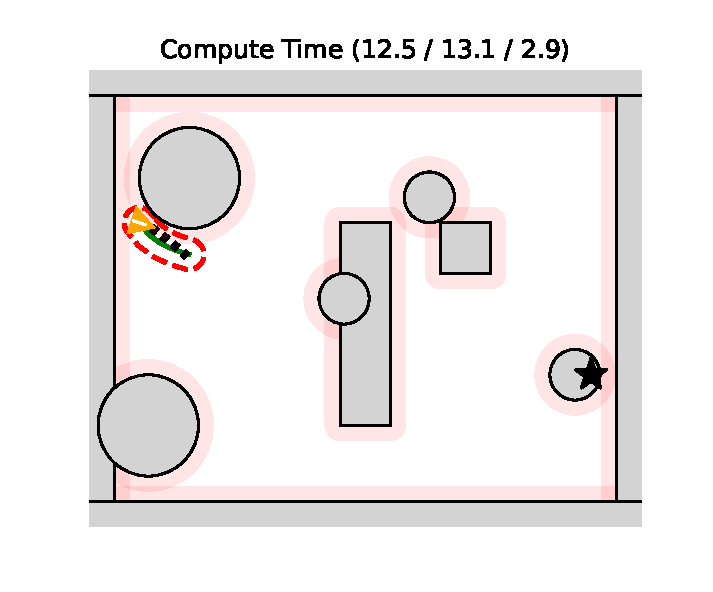
\includegraphics[trim=30 30 30 30,clip,width=0.240\linewidth]{../imgs/08_path_planning/path_1.pdf}
    \hfill
    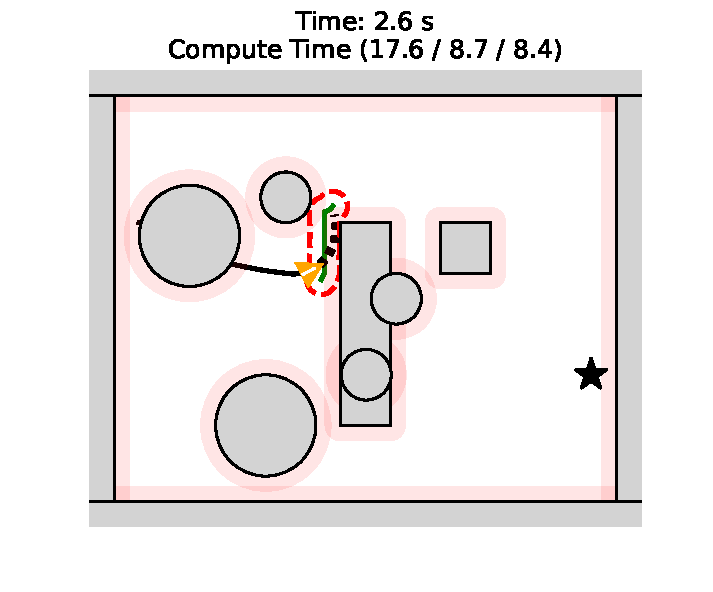
\includegraphics[trim=30 30 30 30,clip,width=0.240\linewidth]{../imgs/08_path_planning/path_2.pdf}
    \hfill
    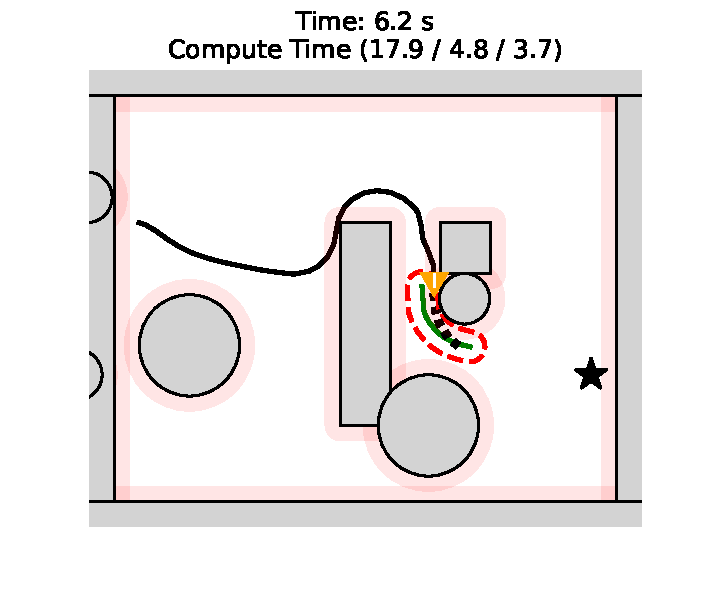
\includegraphics[trim=30 30 30 30,clip,width=0.240\linewidth]{../imgs/08_path_planning/path_3.pdf}
    \hfill
    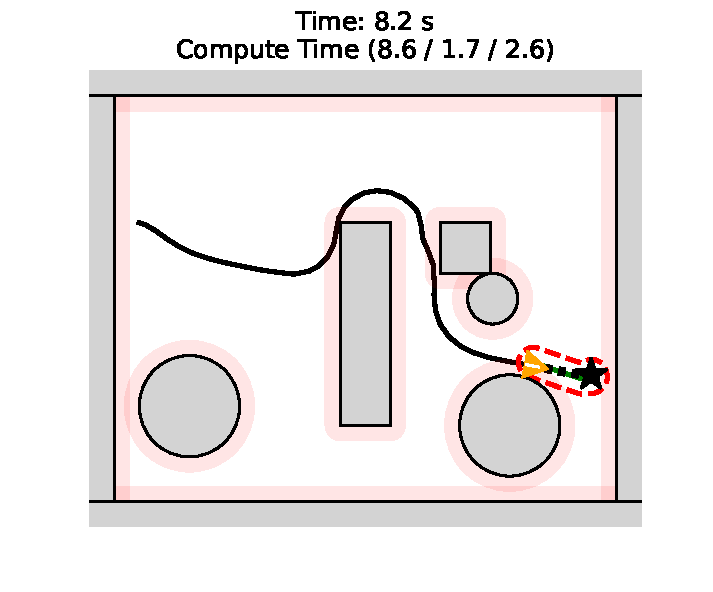
\includegraphics[trim=30 30 30 30,clip,width=0.240\linewidth]{../imgs/08_path_planning/path_4.pdf}
    \caption{Path generation for a unicycle robot with dynamic obstacles and safety guarantees over time (left to right). The robot (yellow arrow) follows the kinematically constrained trajectory (black dashed) while staying inside the safe area (red boundary) of the local desired trajectory (green solid), reaching the goal (star), never colliding with the dynamic obstacles (circles, translating vertically or horizontally). The overall motion is depicted in solid black, while the obstacle safety boundaries are depicted in light red. Generated with \lorem{[Dahlin]}.}
    \label{fig:path_generation}
\end{figure}


\section{TODO: Simulated map}
TODO: just how it's contructed is relevant, but it's just fixed starified rectangles.


\section{Updating map from sensors}
[TODO: expand a bit]
To navigate the cart-robot system in the environment, an obstacle-free path
must be generated. We achieve this in an online fashion, so to account for
dynamic obstacles. Before creating a path, obstacles must be identified and
converted to a useful representation for the planner. We employ LiDAR scanners
to collect distance measurements of the surrounding environment. Then, we
convert these distances to a point cloud and morphologically inflate the points
into circles in the $xy$-plane. A morphological union is then performed so to
gather circles in bigger blobs, which are then simplified in the interest of
computation time for the next step. The starrification algorithm in
\lorem{[Dahlin]} is used to convert the obstacles in \textit{starshaped}
obstacles, which are then further inflated with a clearance radius using
\lorem{[Dahlin]} to create a \textit{tube-path} that guarantees convergence to
the goal pose using the planner in \lorem{[Huber]}.


\section{Localization and navigation}
\section{Localization}
\subsubsection{Odometry}
If you just want to move by 3 meters to test a whole body controller,
and you do not really need to know where on the map this is happening,
you want odometry. If you are interacting with one or few objects in the environment,
and do not need to search for them (ex. you're testing a door-opening controller),
then put QR codes on the object, and localize from vision ---
you do not need to know where these QR code are in the room (or that there even is a room apart
from the space between the robot and the object).

Falls apart in about 10 meters or 1-2 minutes or runtime.

\subsubsection{Maps}
Use someone else SLAM unless this is your explicit focus.

\subsubsection{Localization on maps}
Write or use someone else Kalman filter to bridge between slow localization updates
and fast odometry.

\subsection{Navigation}
You actually just use existing controllers,
the only difference is that the robot model is different.
However, some work better than others,
especially for underactuated platforms.
Assuming this is the case, consider the following controllers:
\begin{itemize}
		\item MPC for trajectory tracking
		\item QP with velocity bounds: TODO: test this better
\end{itemize}

\chapter{Computer vision}
\section{What is an image}
\subsection{RGB}
\subsection{RGBD}
\subsection{Lidar}

\section{AI models}
\subsection{YOLO}
\subsection{Segment anything}


\section{Traditional computer vision}
\subsection{Aruko markers and QR codes}
\subsection{Typical filtering steps}

\chapter{Visualization}

\appendix
\chapter{Hardware}
\label{chapter-hardware}

\section{Supportable hardware}
\label{sec-supportable-hardware}
Any interface to a robot that has a function like
\fbox{\texttt{q = interface.getQ()}} to get the current joint positions
and a function to send velocity commands like
\fbox{\texttt{interface.sendQd(qd)}}
can be made to comply with SMC.
Along with this, one needs to have a URDF of the robot
or manually construct the Pinocchio model.

The requirements are codified contract via 
\fbox{\texttt{AbstractRealRobotManager}}'s 
abstract methods.
This class inherits from AbstractRobotManager,
and exist simply because it has additional methods not needed in simulation
(for simulation we use AbstractSimulatedRobotManager which integrates
joint positions instead of reading them from the real robot).


Here are methods which need to implemented
in the \fbox{\texttt{RealXYZRobotManager}} to get SMC to control a real robot XYZ.
\begin{itemize}
		\item \fbox{\texttt{connectToRobot()}}
		\item \fbox{\texttt{\_updateQ()}}
		\item \fbox{\texttt{sendVelocityCommandToReal()}}
		\item \fbox{\texttt{setInitialPose()}}
		\item \fbox{\texttt{stopRobot()}}
\end{itemize}

The following functions are also made abstract,
but could trivially implemented (ex. just an empty return)
if not available or required:
\begin{itemize}
		\item \fbox{\texttt{connectToGripper()}}
		\item \fbox{\texttt{\_updateV()}}
		\item \fbox{\texttt{setFreedrive()}}
		\item \fbox{\texttt{unSetFreedrive()}}
\end{itemize}


%\subsection{Franka Emika}

\section{Supported hardware}
\subsection{Universal robots' robots}
\subsubsection{Interface used by SMC}
We use the \href{https://sdurobotics.gitlab.io/ur_rtde/introduction/introduction.html}{ur\_rtde}
implementation of the \href{https://www.universal-robots.com/developer/communication-protocol/rtde/}{RTDE protocol}.
It is very straightforward and works exactly as expected for SMC purposes and API.
The particulars can be found in table \ref{table-smc-ur-rtde-interface}.
At a higher level, the robot opens a TCP socket dedicated to the RTDE protocol 
at port 30002(? could be +/- 1 or 2, doesn't matter really).
ur\_rtde creates a client side TCP socket which connects to the robot's RTDE socket.
All socket calls, message serialization etc is handled by ur\_rtde and it works without faults.
Importantly,  ur\_rtde fetches all data from the robot at every time-step,
and stores it in its internal struct. This means that there is no communication
cost to accessing particular data.

On the usage side, despite there being only 1 client side socket, there are 3 classes for using it:
RTDEControlInterface, RTDEReceiveInterface and RTDEIOInterface.
They all share the same socket, and this is just for better code design
(separation of concerns, obvious from the name).

\begin{table}[h!]
		\centering
		\label{table-smc-ur-rtde-interface}
		\begin{tabular}{p{4.5cm} | p{8cm}}
				\textbf{SMC function} & \textbf{How it's achieved with ur\_rtde} \\
				\hline
				connectToRobot() & \begin{itemize}
						\item RTDEControlInterface(args.robot\_ip)
						\item RTDEReceiveInterface(args.robot\_ip)
						\item RTDEIOInterface(args.robot\_ip)
				\end{itemize} \\
				\hline
\_updateQ() & rtde\_receive.getActualQ() \\
				\hline
\_updateV() & rtde\_receive.getActualQd() \\ 
				\hline
sendVelocityCommandToReal() & rtde\_control.speedJ(v, args.acceleration, 1/args.ctrl\_freq)
\newline
\textbf{IMPORTANT:} acceleration is a scalar, same for all joints (effectively).
dt is for how long the robot will try to achieve the prescribe velocity v,
i.e. it's the hangup time for the command. 
We set it to be the specified control frequency (500Hz max).\\
				\hline
\_updateWrench() & rtde\_receive.getActualTCPForce(). 
\newline
\textbf{IMPORTANT:} This returns the unfiltered wrench in the \textbf{base frame} of 
the robot. We immediately map it to the end-effector frame $ T_{ w }^{ e }  $.
Upon the start of every script, we also first collect samples to collect the bias,
and offset it. Despite calling rtde\_control.zeroFtSensor(), there can be bias.
And it builds up quickly. After a few minutes it should be recalibrated
if running a continuous experiment.
The sensor is noisy, our baseline filtering gets reliable wrench readings
if the norm of the wrench is \textbf{at least 2N}.\\
setInitialPose() & rtde\_receive.getActualQ() if connected to the robot
and with --no-real (used to match sim to reality before experiment)\\
				\hline
stopRobot() & first send zeros velocity, then go to freedrive. 
Without going to freedrive, the robot keeps trying to go at zero velocity,
but in actuality keeps moving slowly (collides with something in 5-10min)\\
				\hline
connectToGripper() & gripper dependent, look below if connected with flange to arm's wrist.\\
				\hline
setFreedrive() & rtde\_control.freedriveMode() \\
				\hline
unSetFreedrive() & rtde\_control.endFreedriveMode() \\
				\hline
\_sendTorqueCommand() & is available on UR robots now, but there are
no torque-level controllers in SMC. This is future work.
		\end{tabular}
		\caption{SMC-ur\_rtde interface.}
\end{table}

\subsubsection{An opinionated remark on alternative interfaces}
This remark is a ``heads up'' for those who for whatever reason
have to read UR official documentation.

UR has developed its own programming language for controlling
their robots, called URscript. It is simply a butchered version of Python.
As in, it is literally Python, but heavily constricted (can't install Python packages to it for example),
with premade functions to control the robot.
There are 2 additional sockets to control the robot with remotely.
One accepts entire URscript programs and then executes them.
The other waits for one URscript command at a time, and executes it on completion.

Both of these options are completely useless for the purpose of experimental control engineering
because URscript is not a real programming language.
They are very useful for technicians to safely used the robot with the functionality
developed by UR. This is not SMC's target audience. The target audience are people
who want to test novel controllers.
Avoid non-RTDE interfaces completely. Use available SMC's compliance control, 
or even better, write your own (it will cost you less time and get a better result
than reverse-engineering a URscript program you found.)


\subsubsection{Grippers supported in SMC}
\begin{itemize}
		\item some Robotiq grippers (Hand-E, 2FG), via flange
		\item OnRobot  TwoFg (external cabling)
		\item (soon) Schunk EGK-40 via flange
\end{itemize}

\subsubsection{Notes on integrating grippers connected via the flange}
There are 2 distinct, mutually exclusive options:
\begin{enumerate}
		\item communicate with the gripper directly, with the gripper protocol, over the TCP socket
exposed by the robot
		\item find a URcap for your gripper, and find Python code to interface
			with whatever the URcap expects
\end{enumerate}
\paragraph{Direct communication with the gripper}
The robot opens a TCP socket on port 63352 for direct communication with the gripper.
My understanding is that whatever bytes you send to that socket
will be exactly relayed to the gripper.
There is nothing special about the client side socket you construct.
Typical industrial gripper are very simple from a control standpoint,
and so is communication with them. Namely, the state of the gripper
is likely less than 20 bytes in size. The commands you give it are a few bytes
in length (ex. 1 bytes for target position, 1 for motion velocity, and 1 for grasping force).
My recommendation is to read the gripper's documentation, which has to include
which bytes mean what, and implement the communication protocol directly,
with raw bytes being sent and read. It is very likely you will need to read the gripper's
documentation if you just bought it (preferably you read it \textit{before} you bought it).
(Limited) Experience shows that this is the most stable, set it and forget it way to control the gripper.

\paragraph{URcap solution}
If whoever provides the URcap also provides Python code to interact with it,
this is the best possible solution.
However, chances are that there is no Python code. Be wary if you are determined
to find a ``simple'' workaround. This is a dark path to tread on.
I have seen grippers which provide web interfaces, and people writing Python code
to trigger Javascript to move the GUI sliders.
I suggest toughing it out and writing the raw bytes yourself, that way there is 
at least a clear end in sight. But there is no winning here, only tough labour, or
implementing hacks you wish you can hide and forget, or even worse --- external cabling.


%\subsection{Robots with ROS2 drivers}
\section{Robots with ROS2 drivers}
\label{sec-ros2}
\subsection{An opinionated introduction to ROS}
The text in this subsection assumes ROS2, unless stated otherwise.
Furthermore, its purpose is not to provide documentation to ROS,
which is now decent and can be found \href{https://docs.ros.org/}{here}.
Instead, it is to give you, the reader, the minimal necessary context
necessary to decide whether you want to or have to delve into ROS,
and to provide rationale for how SMC is integrated with ROS.

\paragraph{What is ROS}
ROS, which stands for Robotic Operating System, is the biggest
set of open source robotics software.
Its value proposition is to provide a complete software ecosystem
for a robotics platform. The purpose of having a shared ecosystem
is to provide an as uniform as possible API to the various
components of a robotics system --- thus you need to learn 
only one way to program a robot,
instead of multiple frameworks for each component of a robotic system.
This also makes the integration of all components simpler.
Its key component, the feature
that ties everything together, is a multiprocessing and IPC 
framework called RCL. RCL's value proposition is the alleviation
of the need to write explicit multiprocessing and IPC code,
which can be very demanding to implement properly,
and requires a lot of specific knowledge.


Along with RCL, ROS comes with libraries for various components
of a robotic system: path planning (MoveIt), control (ROSControl), navigation (Nav2), 
all kinds of sensor processing, visualization and so on.
Additionally, there are dedicated wrappers around common software building
systems and Linux workflows. For example, ROS packages are build with Colcon
which is a layer on top of CMake.

For more information, the reader is referred to \href{https://docs.ros.org/}{ROS documentation}.


\paragraph{A good situation to use ROS in}
The bigger and more complex the robotic platform in question, the more 
value can be gained by using ROS. This is because if the robotic system
consist of dozens of sensors, multiple computers and possibly hundreds of threads,
management of all this resources becomes practically impossible
if they do not all operate under the same software architecture. 
This is most obvious when working with mobile platform which need
to perform mapping, localization, planning and control,
and make use of ultrasonic distance sensors, Lidars and cameras 
to achieve their tasks.

\paragraph{A situation where ROS is unnecessary}
However, if one works with a simpler robotic system, like a single
manipulator, a force torque sensor and a camera, writing software wrappers
around hardware drivers to conform to a very generic API yields little reward
as these resources can be easily managed individually.
Furthermore, engineers typically work with a few robotic systems
which do not change too often (they are very expensive)
and which they know inside and out. In such cases
adding additional software overhead and dependencies complicates
both software development and maintenance
for very little added functionality.

\paragraph{What is SMC in the context of ROS?}
Within the ROS ecosystem, SMC could be considered as an alternative to ROSControl.
ROSControl of course has better integration with the rest of ROS,
but it has a cumbersome API which makes implementation of controllers time consuming.
On the other hand, since SMC has all workings of an ecosystem,
it could also be considered as an alternative to ROS which targets 
smaller simpler robotic platforms.
It practise, both options work. Which one to use depends 
on the robotic platform in question.

When prototyping whole-body controllers on mobile robots with manipulators,
having ROS run the Nav2 stack to perform mapping and localization,
while using SMC in place of ROSControl gets the best of both worlds.
Upon the completion of the control engineering task, the final controller
can be re-rewritten into ROSControl API to make it more accessible (ROS is popular).

When working with a single manipulator with a few sensors, SMC covers all bases,
and leads to a more flexible workflow due to its leanness.

In the end, one should weight their options and go for what seems like the least
amount of work, which is of course heavily dependent
on one's prior knowledge an experience. As a rule of thumb,
ROS caters more to people with computer science backgrounds,
while SMC caters more to control engineers.

\subsection{SMC-ROS integration approach}
To interact with ROS2 topics programmatically, publishers and subscribers need to be created in a 
ROS \fbox{\texttt{Node}}. This falls under what a RobotManagerXYZ should do.
Getting data from subscribers is only possible through a callback associated with the subscriber object.
Thus, it is also better to publish commands via a dedicated function and timer
to deal with all topics uniformly.

This stands in opposition to AbstractRobotManager's and ControlLoopManager's expected way of working,
but is inelegantly made to work with some ducktaping. 
The main obstacle is that a RobotManagerXYZNode has simultaneously provide functionality of both
ControlLoopManager and RobotManager.
It has to be a ControlLoopManager because it has to publish likely heterogeneous velocity commands via their publishers,
which is meaningless without computing those commands first.
Since only code execution after spin() can happen in topic callbacks,
control needs to be computed in a callback in the Node. There can be only 1 node
as there can be only 1 RobotManager (which is an input to controllerLoops of course).
It also has to read in the current state of the robot via subscription to various topics,
which is the ownership of RobotManager.

This coupling of control signal computation and communication with the robot is exactly
what SMC is trying to avoid --- SMC assumes a fixed robot interface, and swappable controllers.
Controller swapping in ROS is handled via the ROSControl module. The issue with it is its 
verbosity, which slows down quick development and prototyping of controllers (the key
design objective of SMC).
Fortunately, the ducktaping between the two is neither complicated nor too annoying to use,
and the workflow between the two is interoperable where it needs to be.
More on how a RobotManager is made to be a RobotManagerXYZNode can is 
lower in the text. First we introduce main file structure to start a ROS Node.

\subsubsection{Main file structure}
Any file starting a ROS node HAS TO end with the following lines of code:
\begin{minted}[mathescape, linenos]{python}
def main():
    rclpy.init(args=args) # different than smc's args, more on this later
    robot = RobotManagerXYZNode(args_smc, modes_and_loops)
	modes_and_loops = []]

	...

	robot.setModesAndLoops(modes_and_loops)
    executor = MultiThreadedExecutor() # required
    executor.add_node(robot) # required
    executor.spin() # required

if __name__ == "__main__":
    main()
\end{minted}
\paragraph{Hack 1}
The Node can not be used without the executor, and topics can not be interacted with without a Node.
In other words, the robot can only be interacted with from callbacks in the Node.
This in turn means that all control modes and controllers need to be provided to the Node \textbf{before}
executor.spin() is called.
This is done with \fbox{\texttt{modes\_and\_loops}} which is a list of tuples
of control modes and ControlLoopManagers. 

The list is populated like this:
\begin{minted}[mathescape, linenos]{python}
mode_1 = AbstractRobotManager.control_mode.mode_1
loop_manager_controllerX = controllerX(.., args_smc, robot, run=False)
modes_and_loops.append((mode_1, loop_manager_controllerX))
\end{minted}
Hence, instead of immediately running the controller, the output is
a ControlLoopManager instance with the controller and all it's settings.
How the list of controller is used in the RobotManagerXYZNode is described in the following subsection describing
a Node connecting a particular robot in SMC with the ROS2 ecosystem.

\paragraph{Example main file}
An example main file can be found in 
\newline
\fbox{\texttt{examples/ros/mir\_test.py}}.

\subsubsection{Skeleton of ROS2 node for SMC}
Python supports multiple inheritance. This means
we can write a Node which in addition to inheriting from 
\fbox{\texttt{rclpy.node.Node}},
also inherits from both \fbox{\texttt{AbstractRobotXYZRobotManager}}
and \fbox{\texttt{AbstractRealRobotManager}}.
This way we can write a single Node to interact with the robot,
while preserving as much as possible of the SMC architecture.

\paragraph{Hack 2}
Unfortunately one can not use \fbox{\texttt{\_getQ()}}
and \fbox{\texttt{\_getV()}} commands, as SMC does not expects
those to have inputs, while ROS callbacks have to receive and unpack messages.
Hence, the first hack is to leave those as empty, and have the topic callbacks
write to \fbox{\texttt{\_q}} and \fbox{\texttt{\_v}} instead.
At least they remind you that you need to find the appropriate topics
and write their respective callbacks.
(There are other functional design choices, but I felt this was to
be the least convoluted or ugly).

\paragraph{Hack 3}
The second issue is that \fbox{\texttt{sendVelocityCommandToReal}}
does not make sense for the same reason - commands are to be sent via callbacks,
as now the timing for sending messages has to be done via timers in ROS Node's.
The least API-breaking solution is to have a variable
\fbox{\texttt{\_v\_cmd}} which stores the computed velocity command.
\textbf{BIG TODO:} validate that there are no race conditions
on this variable.


\paragraph{RobotManagerNode example}
Look at 
\fbox{\texttt{python/smc/robots/implementations/heron.py}}.


\subsection{Known issues}
\begin{itemize}
		\item Node overrides SIGINT handling from ControlLoopManager, which is in charge 
				of both stopping the robot and saving logs. 
				\textbf{This is a critical issue which needs a proper solution}.
				The current workaround is to rely on the robot's emergency stop button to stop it,
				and to somehow manually trigger log saving (at the moment there is no fully satisfactory solution).
		\item To read the current robot's pose before running a simulation meant to be as close to reality as possible,
				a Node has to be spun (there is no other way to read from a topic programmatically). 
				There is no convenient way to then change topics to those of a ROS2-supported simulator (ex. Gazebo)
				to emulate the topic calls, or to which to a SimulatedRobotManager from within the Node,
				simply running the controllers without publishing. 
				\textbf{This is a critical issue which needs a proper solution. Convenient
				pre-experiment validating simulations are required to safely perform experiments}.
				It is simply too tempting to skip just precautions in the throws of debugging,
				they have to be quick and painless to be actually used.
		\item Node disables opening of windows, blocking plotter from opening a window to plot in.
				Since this is not critical, no solution has been implemented yet.
		\item ROS2 scripts override argument parsing, making it impossible to provide ``normal'' arguments
				to a Python script (which is what's used in SMC). 
				Due to the mutability of the \fbox{\texttt{args}} object ``arguments''
				can be filled in programmatically, but this is an inconvenient hassle.
\end{itemize}




\subsection{Heron}
\paragraph{TODO 1} verify topics via experiment

\subsubsection{Hardware}
There's MiR mobile platform and a UR5e arm. The MiR platform is differential drive.
It has some Lidar and ultrasonic distance sensors. By default, the arm and the base
can not move together, but there is a specific secret hack to circumvent this.

\subsubsection{Software}
There is a whole ROS2 stack, but some parts require additional work. 
By default you control the robot over WiFi, which comes from an onboard router.
The onboard computer supports putting a whole Docker image on it,
meaning one can easily get the best possible control performance.

Despite the ROS stack, SMC arm control relies on ur\_rtde, just as when there's just the manipulator, 
but calls to ur\_rtde are now in callbacks instead.
This choice has been made as ur\_rtde works perfectly fine, and there is
absolutely no benefit in ROS beyond localization (and the utility of this
for whole-body control testing is already very debatable).

The base is controllable only via ROS though.
Base is controlled with \fbox{\texttt{/cmd\_vel}} which runs at 30Hz.

\subsubsection{Localization}
Look at localization subsection in the navigation section.
Odometry is at \fbox{\texttt{/odometry}} and runs at 60Hz.
There's AMCL for localization, but \textbf{carefully consider} whether you really need it.
If you are simply testing a whole-body controller to open a door for example,
there is absolutely no need for localization whatsoever --- just use odometry.


\subsection{ABB Mobile YuMi}
\paragraph{TODO 1} Rewrite SMCYuMiNode into RealMobileYuMiRobotManagerNode (same way as HeronNode)
\paragraph{TODO 2} Finish the todos in yuminode, delete commented code

\subsubsection{Hardware}
YuMi has 2 7dof arms. The payload on the end-effector is like 0.5kg (super weak).
The mechanical design is such that the first 3 links of the arms are very close
to the torso, so it's very easy to get self-collisions between the elbow and the torso.
In short, the elbows should be on the side of the robot,
and the end-effectors should be in front in almost all cases
(have the range of a person with limited shoulder mobility).

The in-house developed research-level mobile base
is omnidirectional and generally works quite well, 
but with some quirks. Namely,
when the robot stops, the wheels reorient themselves
such that the robot can not be pushed.
A similar kind of in-place re-orientation can happen 
if there is a large change in the angle of the commanded velocity.
These functions are performed by the platform - one commands
the base velocity in twist-form. Direct wheel commands are inaccessible.
Additionally, the base only acts of velocities of a certain minimum norm.
Velocities lower than that are (mostly) discarded.
In total, this means that the motion of base should be a trajectory
of (relatively) low curvature, and traversed at a speed
over the minimum. In other words, in continuous operation the robot
is closer to a differential drive. The omnidirectionality is useful
for going in an arbitrary direction from a stationary position.
TODO: None of this is explicitly modelled in YuMiRobotManager,
and it really should be for experiments to be successfully designed
(you can't eyeball your way around this, it has to be modelled).


\subsubsection{Software on the robot}
The robot has a full ROS2 stack.
ROS connects to something called EGM which
is a common external-control controller, i.e. it just listens
to incoming velocity commands and then executes
them with a proprietary inner controller. This is referred to as EGM mode on the robot.
EGM is super annoying (randomly stops working, so need to reset it 
etc). The ROS driver is equally as annoying. Avoid this robot if you have other options,
unless you like restarting everything (5ish min process) every half hour.

The robot has an $f_{ \text{ctrl} } \approx  $60Hz interface for full-body velocity control,
which is a combination of individual velocity ``controllers'' for the base, 
the torso pillar (which we don't use) and the mobile base.

For the most part, the communication with the robot goes over 5G WiFi in the lab,
meaning no code needs to be installed on the robot, but there are occasional lag spikes
leading to loss of control for (eyeballed) 0.2-0.5 seconds. 
[Marko's estimate is that ] This kind of interfacing is just barely acceptable
if the control is slow and conservative. It is possible to install additional ROS2
packages on the robot, but [by Marko's estimate] installing the control software stack
is an ill-advised adventure as there is no Docker on the robot.

From a control perspective,
the specific topics to interact with the robot are:
\begin{itemize}
		\item (namespace)/platform/joint\_states - used
				to fetch current joint angles (all of them).
				Uses sensor\_msgs.msg.JointState as message format,
				and it's just a vector of all joint angles.
		\item (namespace)/platform/joints\_cmd - used
				to send a velocity command to all 
				joints. Also uses  sensor\_msgs.msg.JointState
		\item (namespace)/platform/odometry - odometry topic.
				Good enough for small experiments,
				but there is AMCL for actual localization
				(0.5Hz though, you need a filter to make use of
				it).
\end{itemize}

\subsubsection{Concrete steps to use the robot}
TODO document how to operate mobile yumi in vasteros 
(sequence of buttons to press to restart it after it craps out),
how to start Rviz and what to click in it to start EGM etc.

\paragraph{In code}
ATM in python/smc/multiprocessing/smc\_yumi\_node.py,
will get rewriten to be like heron
and moved to python/smc/robots/implementations/mobile\_yumi.py

\subsection{Sleipner + YuMi (SLuMi)}
TODO
It's ROS1
things to do
1. turn power on on robot. first 


\section{Robot connection (network) checklist}
\begin{enumerate}
	\item Is the ethernet cable plugged in (are laps blinking) / are you connected to wifi?
	\item Do you know the IP address of the robot?
\begin{itemize}
	\item Do you know your own IP address on LAN?
		Use nmcli, ifconfig, or ip addr to find it. 
		Also note the interface for this IP. Is it ethernet or wifi? Do you know which one you want?
	\item Find all IPs on a network with arp-scan. 
		You might have to specify the network interface to get output (ex. eth0). 
		You also might have to run this as root (put sudo in front of command)
		Example:
		\newline
		arp-scan 192.168.0.1/24 -I eth0
\end{itemize}
\item Is the robot actually connected to the network? Send it a ping with ping ROBOT\_IP.
\item If on Docker, are you sure you share your host network with the Docker container?
	Do all network checks in this list on both your host and inside the Docker container.
	If your OS does not support --net=host on Docker, make sure you're forwarding the necessary ports.
\item Are you sure the robot is ready to receive commands?
\begin{itemize}
\item Is the robot set to "remote control" or whatever similar setting for you to be able to connect to it?
\item Is the robot in "emergency stop mode"?
\item Are the robot's motor on/initialized?
\end{itemize}
\item Are you sure can connect to the robot? 
\begin{itemize}
	\item Try ssh-ing into it/ open its dashboard in WEB/whatever else to make sure connection is fine, and not some problem with 
		the control port, or the driver. 
\end{itemize}
\item Are you sure can use the remote-control interface/robot driver? 
\begin{itemize}
	\item Did the previous interface exit cleanly? The socket might not have been cleaned up. Try running again. 
		Look at the terminal for specific errors. Try running again.
	\item If using ROS, are you sure all topics are brought up? Do topic list. Then do topic echo on all of them.
\end{itemize}
\item Remove all bells and whistles to test just connection to the robot, maybe just one of the following is the problem:
\begin{itemize}
	\item Skip connecting to the gripper, if any.
	\item Skip parts of the robot. Say on a mobile manipulator, connect to just the arm. Then just the base. 
	\item Skip initializing f/t sensors, if any.
	\item Skip initializing the camera, if any.
	\item If on ROS, do the smallest possible bringup.
	\item Use the simplest possible control example (I always do a point-to-point clik).
\end{itemize}
\item Reboot the robot, run through all the steps again.
\item Reboot your computer, run through all the steps again.
\item Use a different computer, run through all the steps again.
\item Are you using a 1-1 to connection to the robot, or is it going through some LAN in your lab? 
	This intermediary might be the culprit.
	Switch to a 1-1 connection (network is just your computer and the robot, create new fixed connection),
	i.e. plug the ethernet cable directly from the robot into your computer.
	If the robot itself has a router, switch etc, try skipping over it and go directly to the robot.
	Maybe this router/something else has to run DHCP, and you have to let it assign you an IP.
	Try both a fixed IP and let whatever assign the IP to you. The same goes for the robot itself.
	(had a gripper that had to run it's DHCP, and everything obey the gripper).
\item Disable (all) firewall(s) on your computer, if any, try again 
	(had a Windows computer which did not allow socket.bind() period, due to idk what).
\item Maybe something else is preventing socket binding/listening. ssh into the robot. Try connecting with netcat. 
	nc -kl 0.0.0.0 7777 on robot, try nc ROBOT\_IP 7777 on your computer. This should be an echo server.
	Try nc -kl ROBOT\_IP 7777 on robot also. Try using different ports.
	Make sure it works the other way around, i.e. nc -kl on your machine , nc from robot (-l is listening, meaning that's the server).
\item If you got to here, you can connect to the robot and the interface doesn't work for whatever reason.
	Try putting your control code onto the robot's computer, run it from there. First just try the driver from the robot itself.
\item Send an email/open a github issue to whoever gave you/wrote the interface to the robot, give them all the error logs
	and convince them it's not something in the connection or something preventing connections on your computer.
\end{enumerate}


\chapter{Simulation}
Here by simulation we mean physics simulation. 
Since SMC does not have an API connection to a physics simulator,
this section won't be about its details.
Instead, we'll briefly cover 
\begin{itemize}
		\item what is the point of physics simulation
		\item how to test controller correctness without a physics simulator
		\item how to prepare for a hardware experiment
		\item how to integrate SMC with a physics simulator
\end{itemize}

\subsection{What is the point of physics simulation?}
TODO

\subsection{How to test controllers?}
TODO


\subsection{How to prepare for a hardware experiment}
TODO

\subsection{Integrating SMC with a physics simulator}
TODO




\printbibliography
\end{document}
